\documentclass[letterpaper,10pt]{book}
% Change to 10 pt
\usepackage{pdfpages}
\usepackage{morewrites}			% to counteract the no write space problem
\setcounter{tocdepth}{5}

\usepackage[framemethod=TikZ]{mdframed}

\usepackage{fancyhdr}

\usepackage{paralist}
\usepackage{amsmath}
\usepackage{amsfonts}
\usepackage{amssymb}
\usepackage{graphicx}

\usepackage{datetime}
%\usepackage{ulem}

%\usepackage[nottoc]{toobibind}

\usepackage[inline]{enumitem}

% Outer margin at 2.50 is exactly correct to fit the ``corruption alert'' tables
\usepackage[inner=1.0in, outer=2.50in, top=2.54cm,bottom=2.54cm, marginparwidth=2.25in]{geometry}

\usepackage{marginnote}
\usepackage{longtable}
\usepackage{booktabs}
\usepackage{xcolor}

\usepackage{soul}

\usepackage{marginnote}
\usepackage{imakeidx} 
\usepackage[
	backref=true,
	style=numeric,
%	citestyle=numeric,
	backend=bibtex
	]{biblatex}
\usepackage[driverfallback=hypertex,colorlinks=True]{hyperref}
\usepackage{cleveref}

\makeindex[name=scripture,columnsep=20pt, columnseprule=True,columns=3, title=Scripture References]
\makeindex[name=speaker,columnsep=20pt, columnseprule=True,,columns=2, title=Sermon Creator]
\makeindex[name=series,columnsep=20pt, columnseprule=True,,columns=2, title=Sermon Series]
\makeindex[name=date,columnsep=20pt, columnseprule=True,columns=2, title=Sermon Date]

\makeindex[name=event,columnsep=20pt, columnseprule=True,columns=2, title=Event]

\makeindex[name=topic,columnsep=20pt, columnseprule=True,columns=2, title=Topic]
\makeindex[name=AWIP,columnsep=20pt, columnseprule=True,columns=3, title=All Words in Passage]
\makeindex[name=NWIV,columnsep=20pt, columnseprule=True,columns=3, title=Number of Words in Verse]
\makeindex[name=PNIP,columnsep=20pt, columnseprule=True,columns=3, title=Proper Names in Passage]
\makeindex[name=PEIP,columnsep=20pt, columnseprule=True,columns=2, title=Prophetic Events in Passage]


\makeindex[name=TWPAQ,columnsep=20pt, columnseprule=True,columns=1, title=13-Word Phrases and Quotes]
\makeindex[name=PFTTIS,columnsep=20pt, columnseprule=False,columns=3, title=Phrases found 13 times in scripture]
\makeindex[name=WFTTIS,columnsep=20pt, columnseprule=False,columns=3, title=Words found 13 times in scripture]
\makeindex[name=WFITV,columnsep=20pt, columnseprule=False,columns=3, title=Words found in exactly 13 verses]
\makeindex[name=EVENTS,columnsep=20pt, columnseprule=False,columns=2, title=Sermon Log by Place]
\makeindex[name=QUESTIONS,columnsep=20pt, columnseprule=False,columns=2, title=Bible Questions]

\makeindex[name=DOCTRINES,columnsep=20pt, columnseprule=False,columns=2, title=Doctrines]

\makeindex[name=SONGS,columnsep=20pt, columnseprule=False,columns=1, title=Songs]
\makeindex[name=LOCATION,columnsep=20pt, columnseprule=False,columns= 2, title=Location]
\makeindex[name=FACEBOOK,columnsep=20pt, columnseprule=False,columns=2, title=Facebook]

\makeindex[name=DEVOTIONAL,columnsep=20pt, columnseprule=False,columns=1, title=Devotionals]

\pagestyle{fancy}
\fancyhf{}
\fancyhead[LE,RO]{\today}
\fancyhead[RE,LO]{Notes, Outlines, Comments}
\fancyhead[CE,CO]{-page \thepage  - }

\fancyfoot[CO,CE]{\leftmark}
%\fancyfoot[LE,RO]{CSCE 692, HW1}

\title{DBR\\
Daily \\ Reads}
\author{Keith Anthony \\
\today }
%\title

%+/ffffff +   \pagenumbering{gobble}

\bibliography{Bibliographies/All20220108}

%%%%% TWEAKS:
%%% - distance from fcolorbox frame to text
\setlength{\fboxsep}{1.0pt}

\usepackage[utf8]{inputenc}
\usepackage{tikz}

%%%%%%%%%%%%%%%%%%%%%%%%%%%%%%%%%%%%%%%%%%%%%%%%%%%%%%%%%%%%%%%%%%%%%%%%%%%%%%%%

\begin{document}

\begin{titlepage}

% Set the text of the page to right-aligned until \end{flushright}
\begin{flushright}
\rightskip=-2.5cm

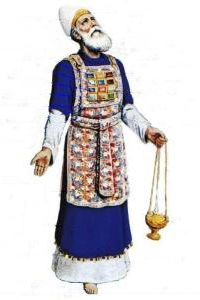
\includegraphics[width=50mm,scale=1.5]{Melchisedec.jpg}
\vspace{0.4in}

% Create a title for the document and write it in bold font
\LARGE{\textbf{\date}}
\linebreak

\vspace{0.5in}


\begin{flushleft}
\LARGE{Psalms 1-25\\}\vspace{0.25in}
\LARGE{Notes, Outlines, Comments}
\end{flushleft}

% write in large letters
%\large{Free webservices and apps}

% Skip some space
\vspace{0.6in}

%\large{Documentation}
% Skip some space

\bigskip

\normalsize{Xenia, Oh.\\}
\normalsize{created: \today}

% Skip some space
\vspace{1.3in}

\end{flushright}
% End the title page
\end{titlepage}

%\titlehttps://www.overleaf.com/project/60d732302fc633866943c9d2JE

\newpage 

\tableofcontents\hypertarget{TOC}{}
\listoffigures
\listoftables

\hyphenation{A-bim-e-lech bre-thren E-phra-im  Gib-e-o-nites Jer-u-sa-lem through-out Phil-i-stines The-o-phil-us Am-a-le-kites ven-geance Mesh-el-e-mi-ah onan-ism Phar-a-oh Py-thon thoughts grev-ous-ness Hach-a-liah adul-ter-er Shad-rach}

%\fcolorbox{black}{bone}{TEXT}
%%%%%%%%%%%%%%%%% EXTRA COLORS
%%%%%%%%%%%%%%%%% EXTRA COLORS
%%%%%%%%%%%%%%%%% EXTRA COLORS
\definecolor{champagne}{rgb}{0.97,0.91,0.81}
\definecolor{bone}{rgb}{0.89,0.85,0.79}

\definecolor{ForestGreen}{rgb}{0.00,0.29,0.098}
\definecolor{GIVING}{cmyk}{1,0.0,0.72,.1}

\definecolor{MLPE}{cmyk}{1,1,0,.45}
\definecolor{SOCCER}{cmyk}{.77, 0, .42, .49}
\definecolor{PAYBILL}{cmyk}{0,0.83,0.76,0.07}
\definecolor{SERMON}{cmyk}{.14,.9,0,.30} % aka seance \href{http://www.flatuicolorpicker.com/purple-cmyk-color-model/}{seance}
\definecolor{BIBLE}{cmyk}{0,.17,.74,.17}
\definecolor{WORKBLUE}{cmyk}{1, .5, 0, .6}
\definecolor{myOrange}{cmyk}{0, .4, .98, .03}
\definecolor{myTan}{cmyk}{0.0,.07,.17,.10}
\definecolor{myRed}{cmyk}{0,1,1,0}
\definecolor{myWhite}{cmyk}{0,0,0,0}
\definecolor{BLUESoD}{cmyk}{.97,.84,0,.04}
\definecolor{WHITE}{cmyk}{0,0,0,0}
\definecolor{OLDGOLD}{cmyk}{0.05,0.3,1.00,0}
\definecolor{CASTLETON}{cmyk}{1,0,0.31,0.66}
\definecolor{cadmiumgreen}{rgb}{0.0, 0.42, 0.24}
\definecolor{jungle}{rgb}{0.203,0.4882,0.1718}
\definecolor{MYGOLD}{rgb}{1,.84,0}

\definecolor{MYLIGHTGRAY}{rgb}{.85,.85,.85}

\definecolor{codegreen}{rgb}{0,0.6,0}
\definecolor{codegray}{rgb}{0.5,0.5,0.5}
\definecolor{codepurple}{rgb}{0.58,0,0.82}
\definecolor{backcolour}{rgb}{0.95,0.95,0.92}



\mdfdefinestyle{MyFrame}{%
    linecolor=blue,
    outerlinewidth=2pt,
    roundcorner=5pt,
    innertopmargin=\baselineskip,
    innerbottommargin=\baselineskip,
    innerrightmargin=10pt,
    innerleftmargin=10pt,
    backgroundcolor=gray!25!white}


\mdfdefinestyle{MyFrame2}{%
    linecolor=black,
    outerlinewidth=2pt,
    roundcorner=5pt,
    innertopmargin=\baselineskip,
    innerbottommargin=\baselineskip,
    innerrightmargin=10pt,
    innerleftmargin=10pt,
    backgroundcolor=yellow!25!white}



%\input{PFTTIS}
%\input{WFTTIS}
%\input{WFITV}

%
%\newpage
%\begin{figure}
%\begin{center}
%\includegraphics[scale=.7, angle=0]{05OT-Deuteronomy/References/AndrewSmithDeuteronomyTimeline.png}
%\caption[Deuteronomy Timeline by Andrew Smith]{Deuteronomy Timeline by Andrew %Smith}
%\label{fig:Deuteronomy Timeline by Andrew Smith}
%\end{center}
%\end{figure}

\newpage
\begin{figure}
\begin{center}
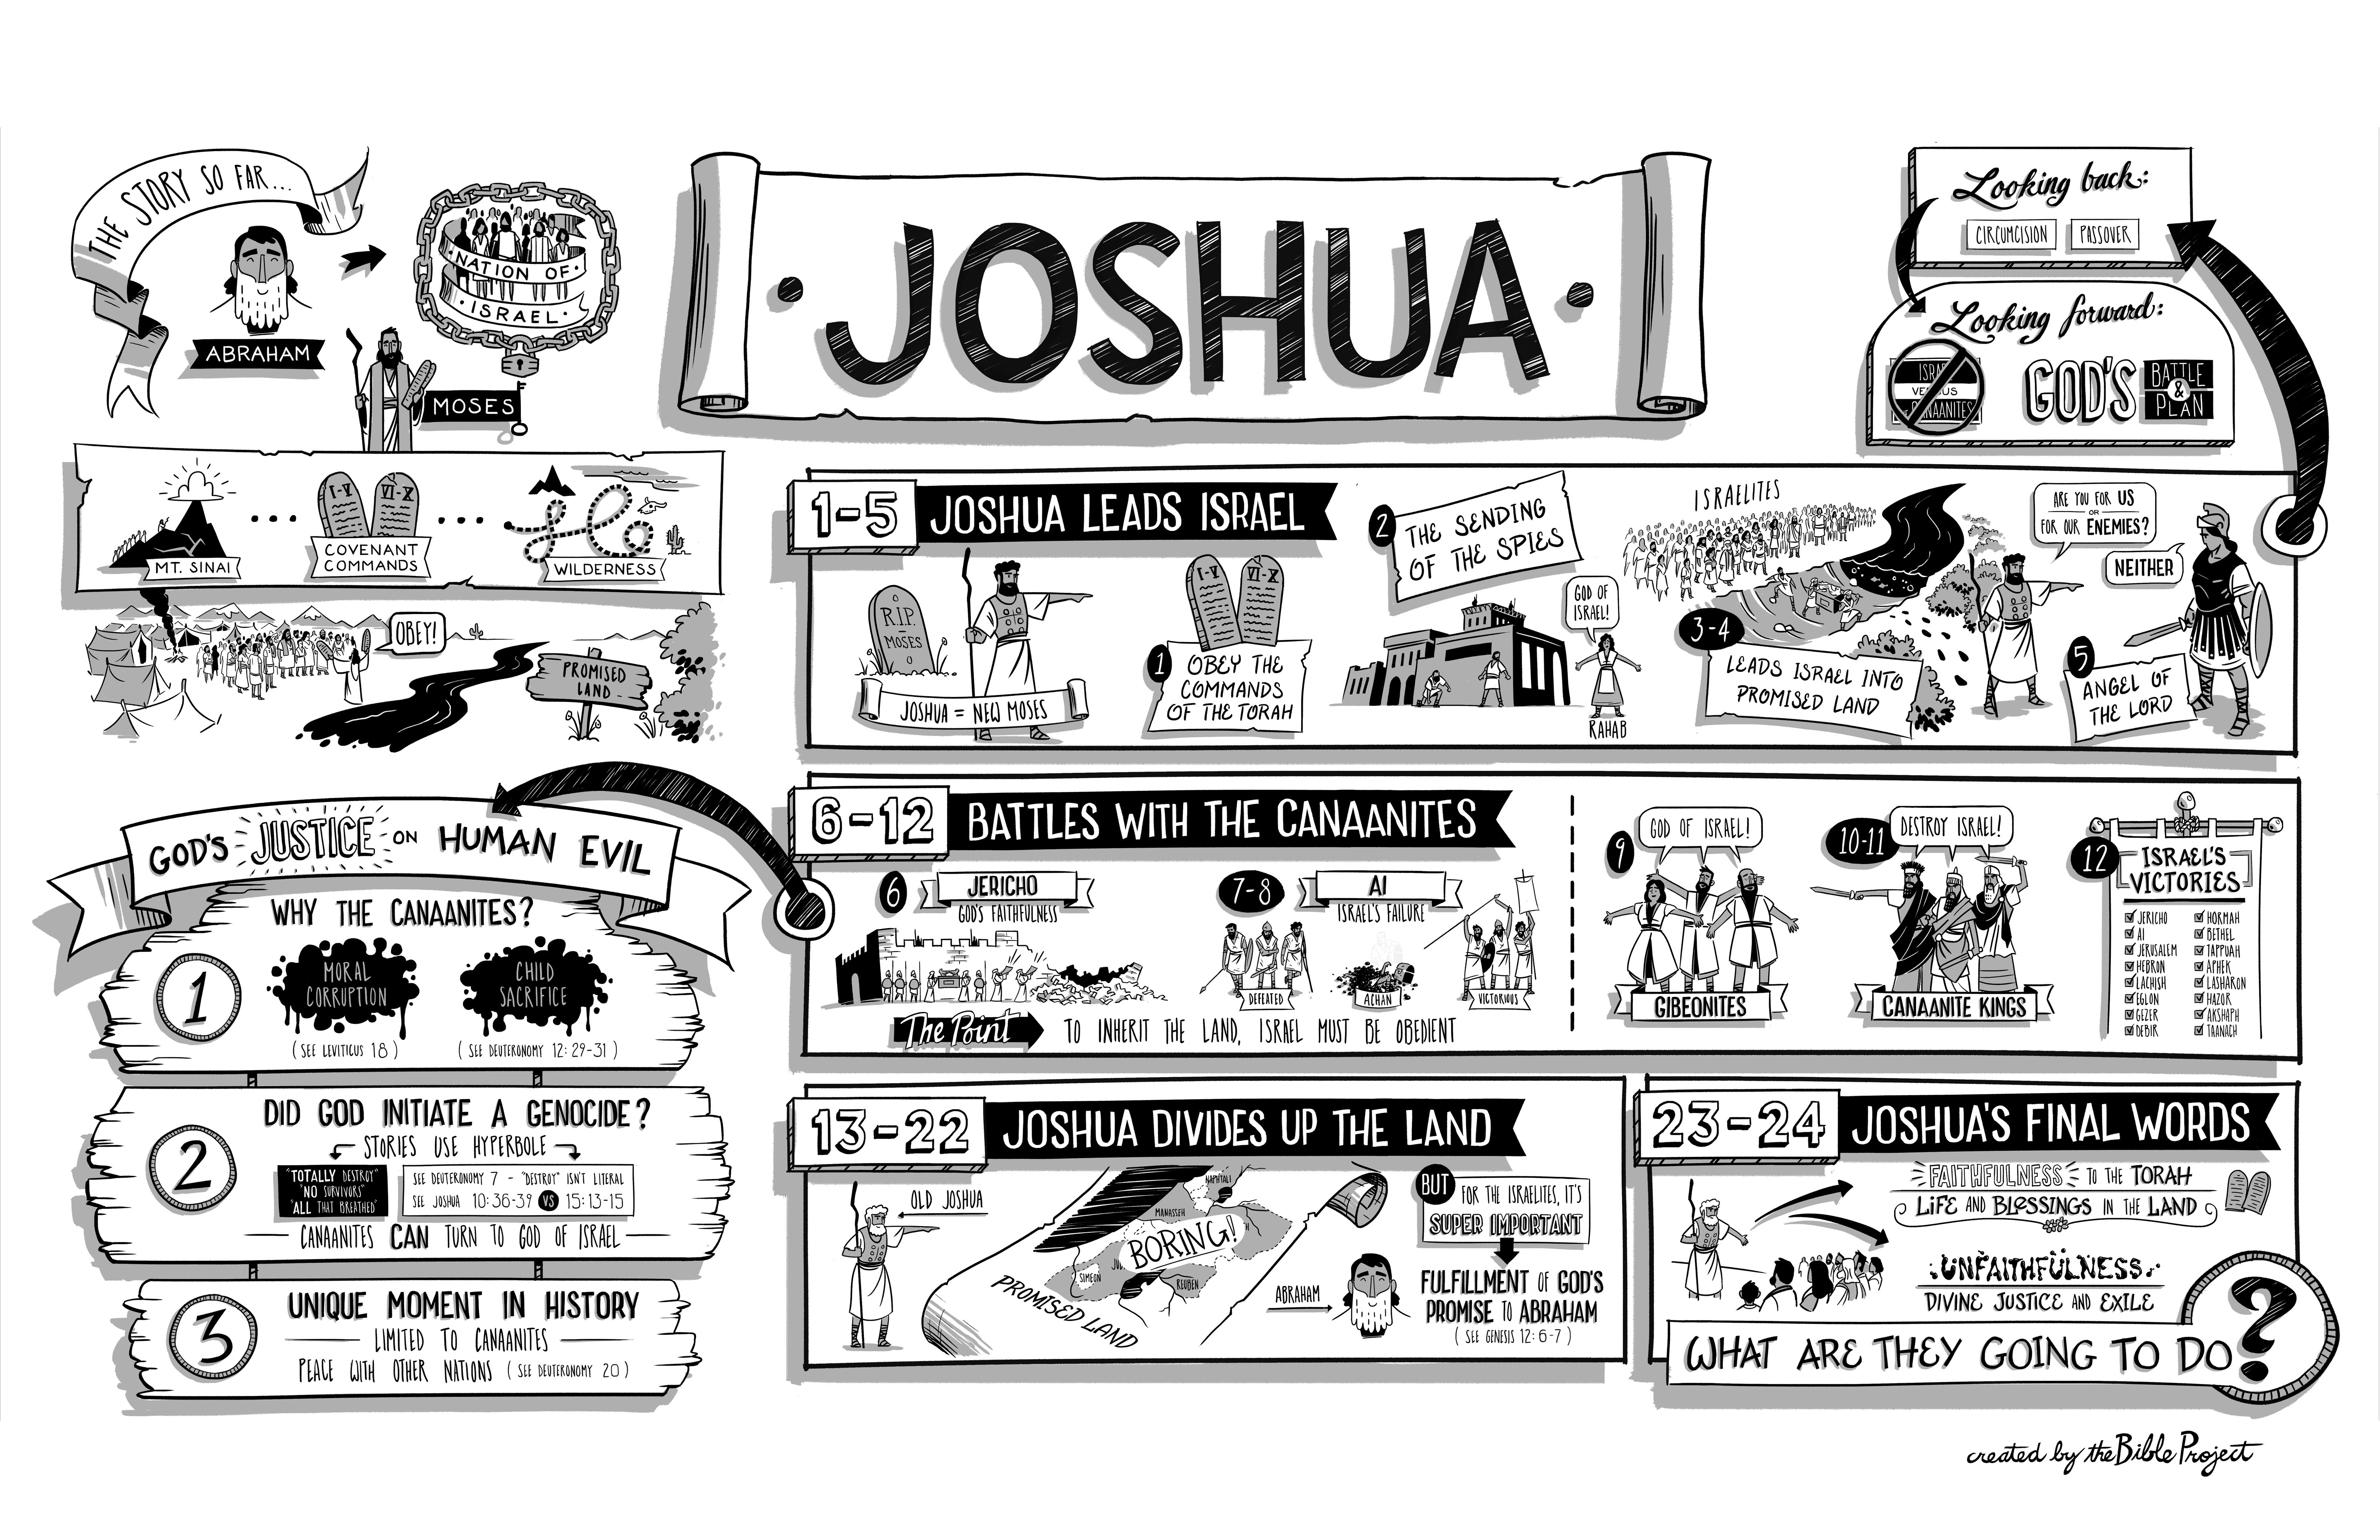
\includegraphics[scale=0.5, angle=90]{06OT-Joshua/References/1.BibleProject-Joshua.jpg}
\caption[Joshua from the Bible Project]{Joshua from the Bible Project}
\label{fig:Joshua from the Bible Project}
\end{center}
\end{figure}

\newpage
\begin{figure}
\begin{center}
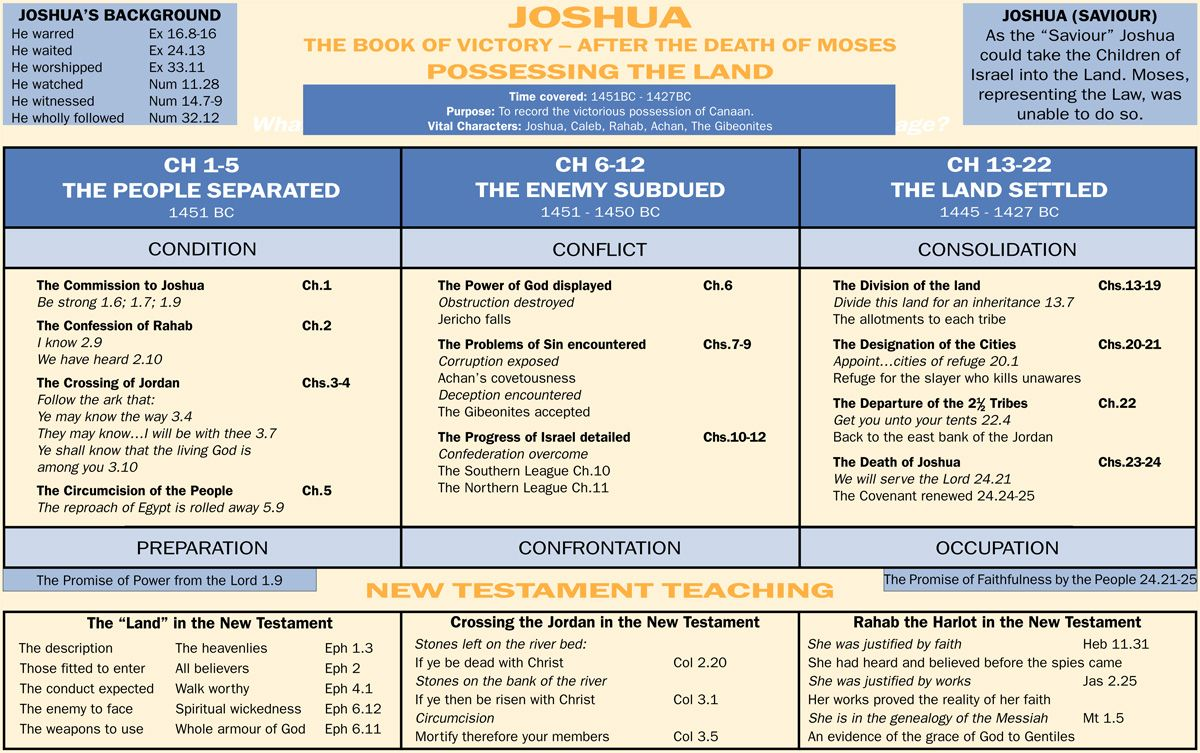
\includegraphics[scale=0.5, angle=90]{06OT-Joshua/References/2.JohnGrant-Joshua.jpg}
\caption[Joshua from John Grant]{Joshua from John Grant}
\label{fig:Joshua from John Grant}
\end{center}
\end{figure}

\newpage
\begin{figure}
\begin{center}
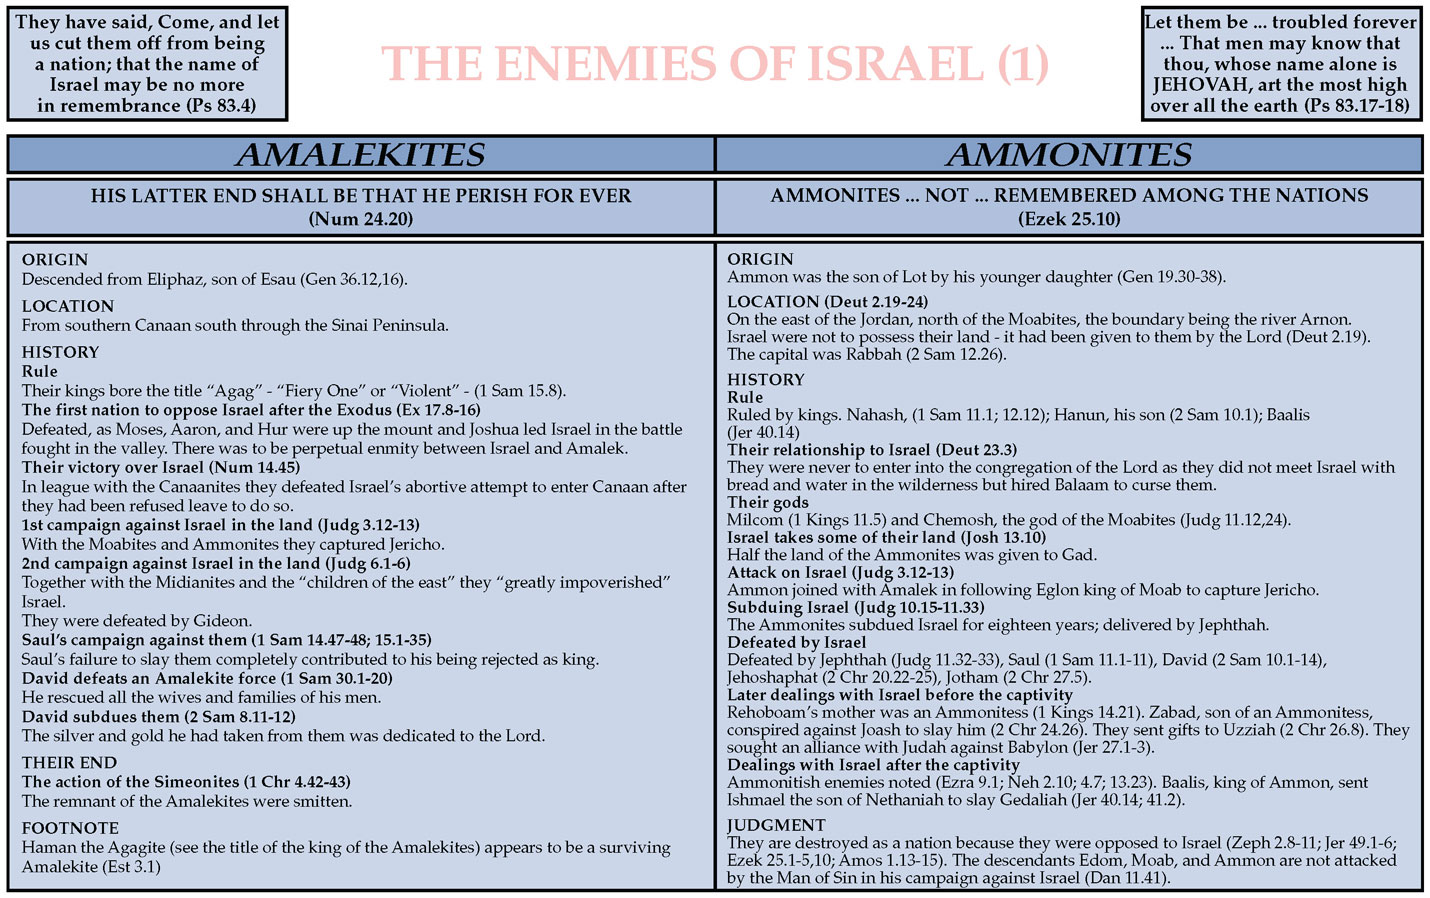
\includegraphics[scale=0.4, angle=90]{06OT-Joshua/References/3.EnemiesOfIsrael1.jpg}
\caption[Enemies of Israel 1]{Enemies of Israel 1}
\label{fig:Enemies of Israel 1}
\end{center}
\end{figure}

\newpage
\begin{figure}
\begin{center}
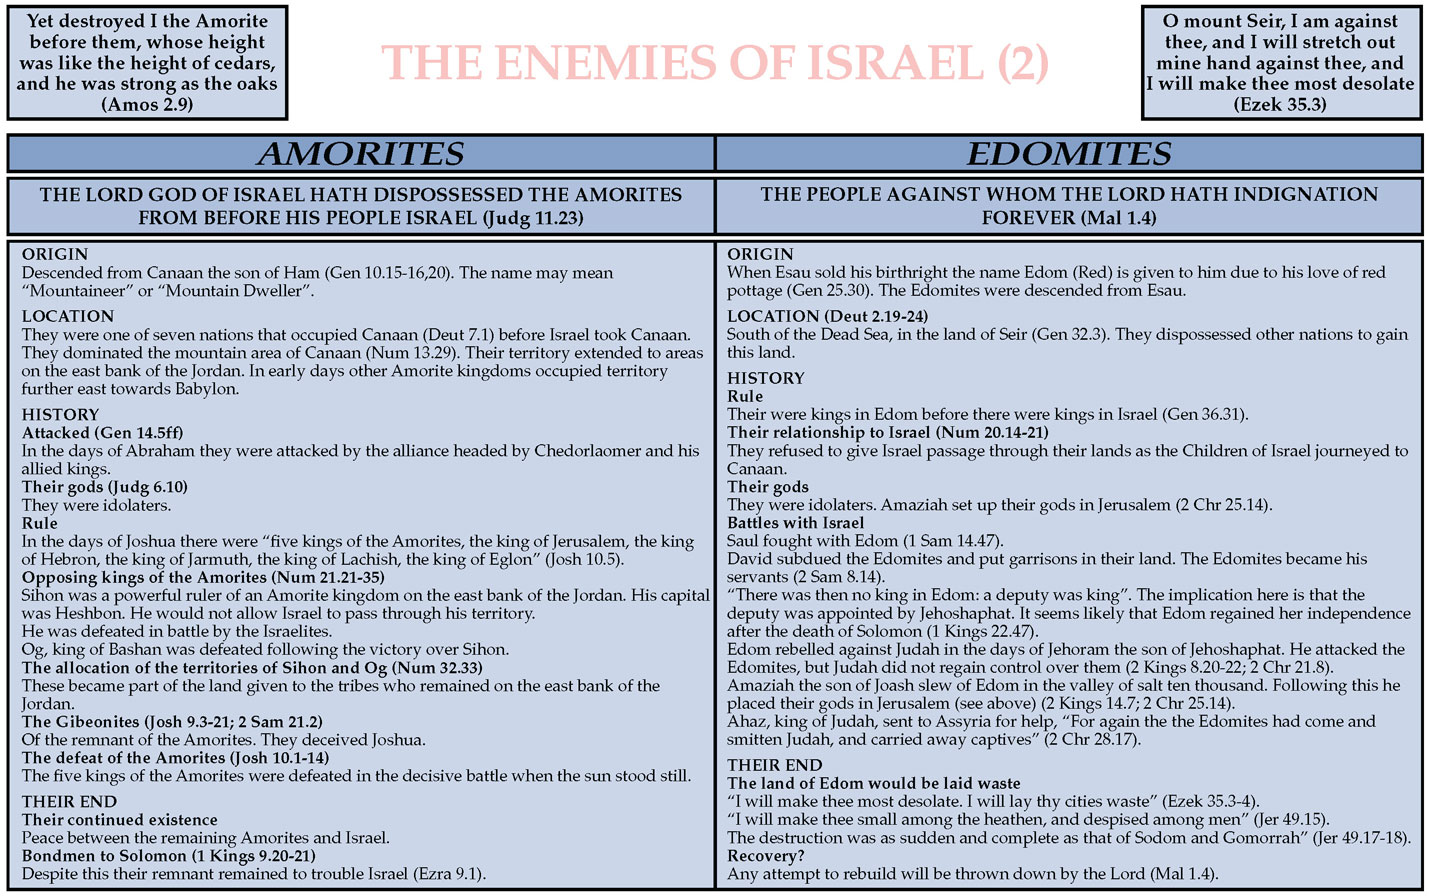
\includegraphics[scale=0.4, angle=90]{06OT-Joshua/References/4.EnemiesOfIsrael2.jpg}
\caption[Enemies of Israel 2]{Enemies of Israel 2}
\label{fig:Enemies of Israel 2}
\end{center}
\end{figure}

\newpage
\begin{figure}
\begin{center}
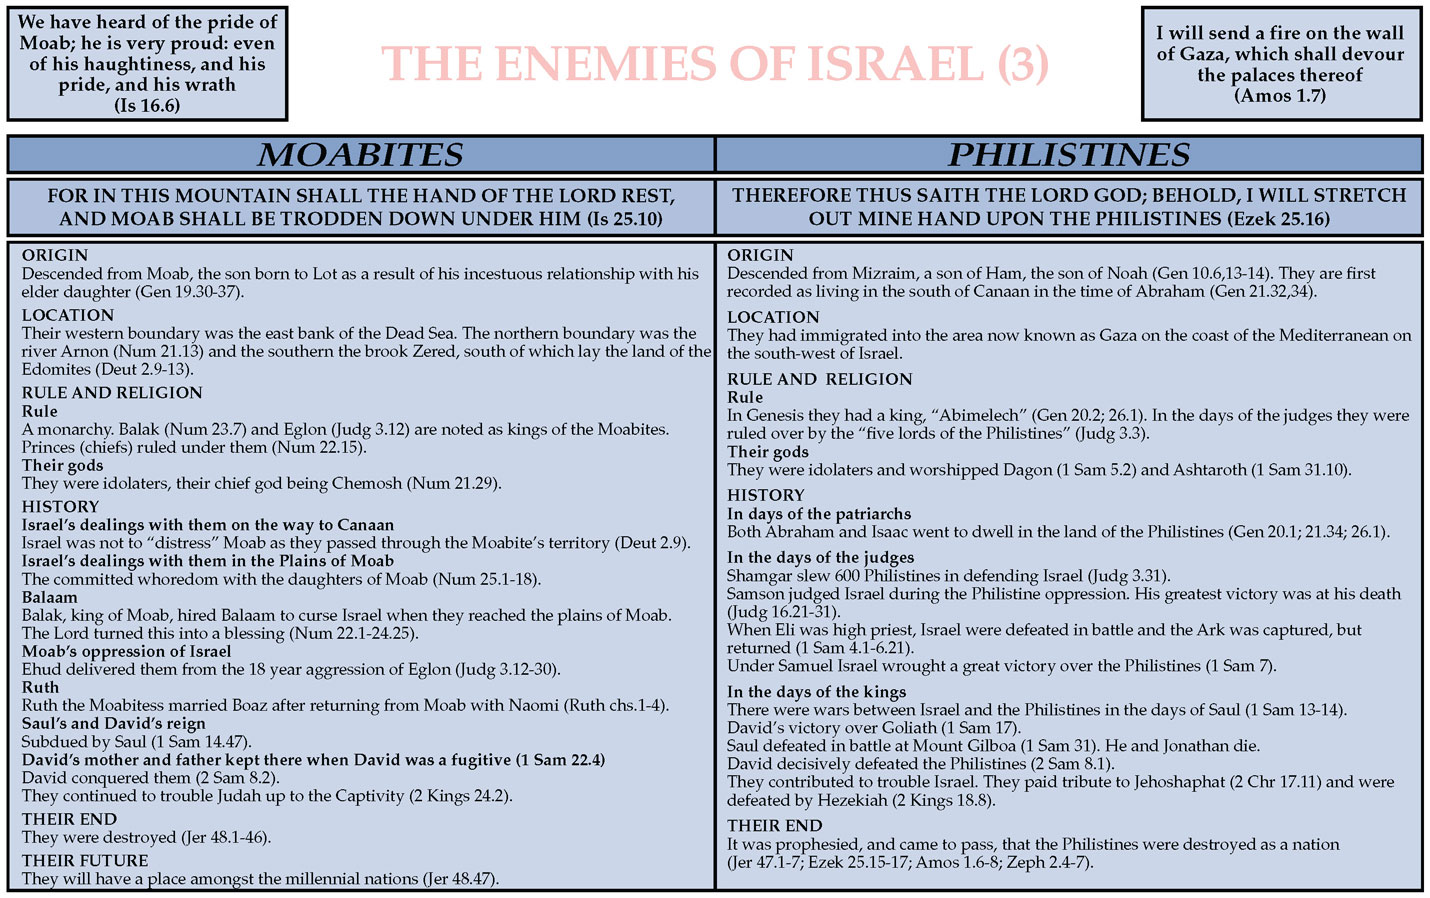
\includegraphics[scale=0.4, angle=90]{06OT-Joshua/References/5.EnemiesOfIsrael3.jpg}
\caption[Enemies of Israel 3]{Enemies of Israel 3}
\label{fig:Enemies of Israel 3}
\end{center}
\end{figure}

\newpage
\begin{figure}
\begin{center}
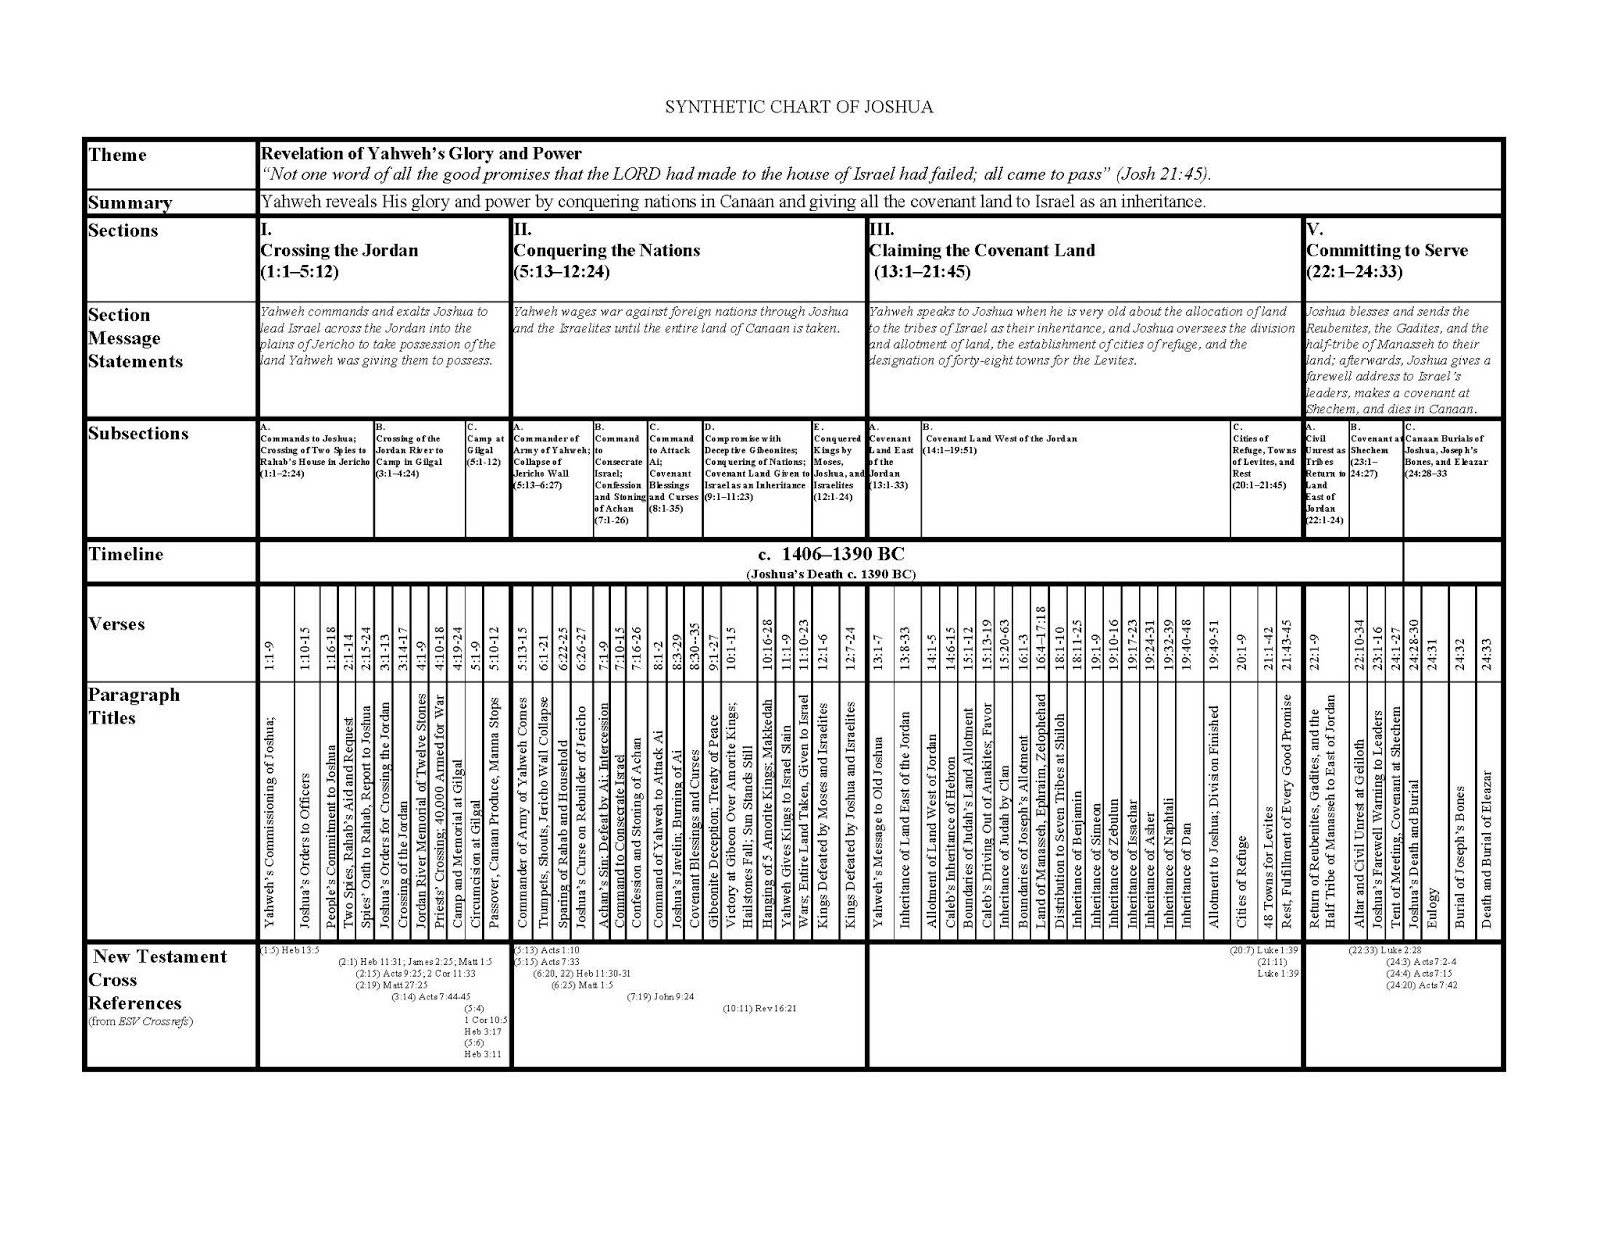
\includegraphics[scale=.4, angle=90]{06OT-Joshua/References/6.SyntheticChartofJoshua.jpg}
\caption[Synthetic Chart of Joshua]{Synthetic Chart of Joshua}
\label{fig:Synthetic Chart of Joshua}
\end{center}
\end{figure}


\newpage
\begin{figure}
\begin{center}
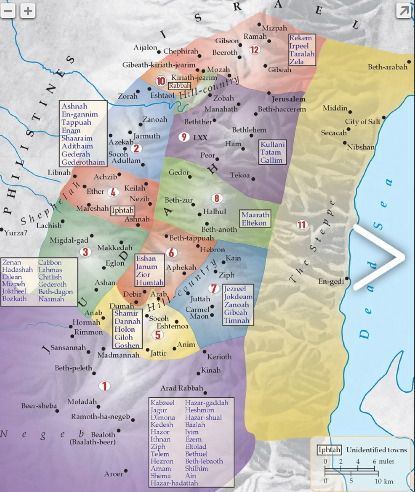
\includegraphics[scale=1, angle=0]{06OT-Joshua/References/7.WestSideOfDeadSea.jpg}
\caption[The West Side of the Dead Sea]{The West Side of the Dead Sea}
\label{fig:The West Side of the Dead Sea}
\end{center}
\end{figure}


\newpage
\begin{figure}
\begin{center}
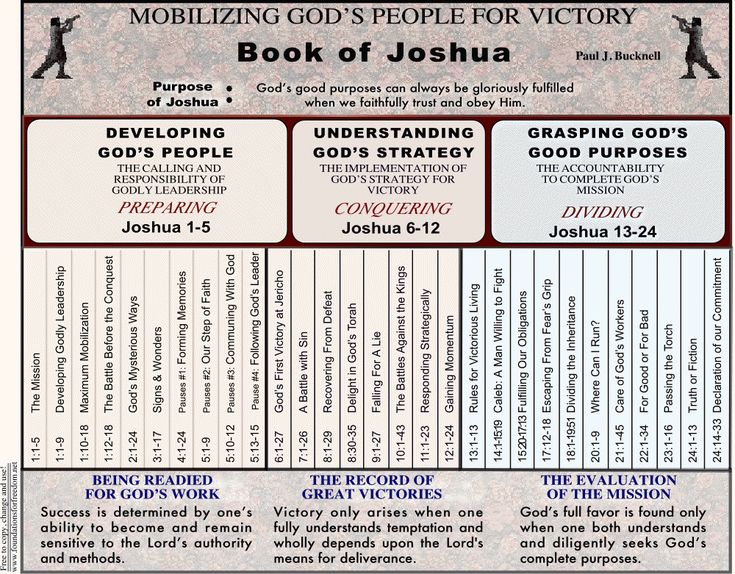
\includegraphics[scale=0.75, angle=90]{06OT-Joshua/References/8.Bucknell-Joshua.jpg}
\caption[Joshua from Bucknell]{Joshua from Bucknell}
\label{fig:Joshua from Bucknell}
\end{center}
\end{figure}


%\newpage
%\begin{figure}
%\begin{center}
%\includegraphics[scale=2, angle=90]{06OT-Joshua/References/9.Jensen-Joshua.png}
%\caption[Joshua from Jensen]{Joshua from Jensen}
%\label{fig:Joshua from Jensen}
%\end{center}
%\end{figure}


\newpage
\begin{figure}
\begin{center}
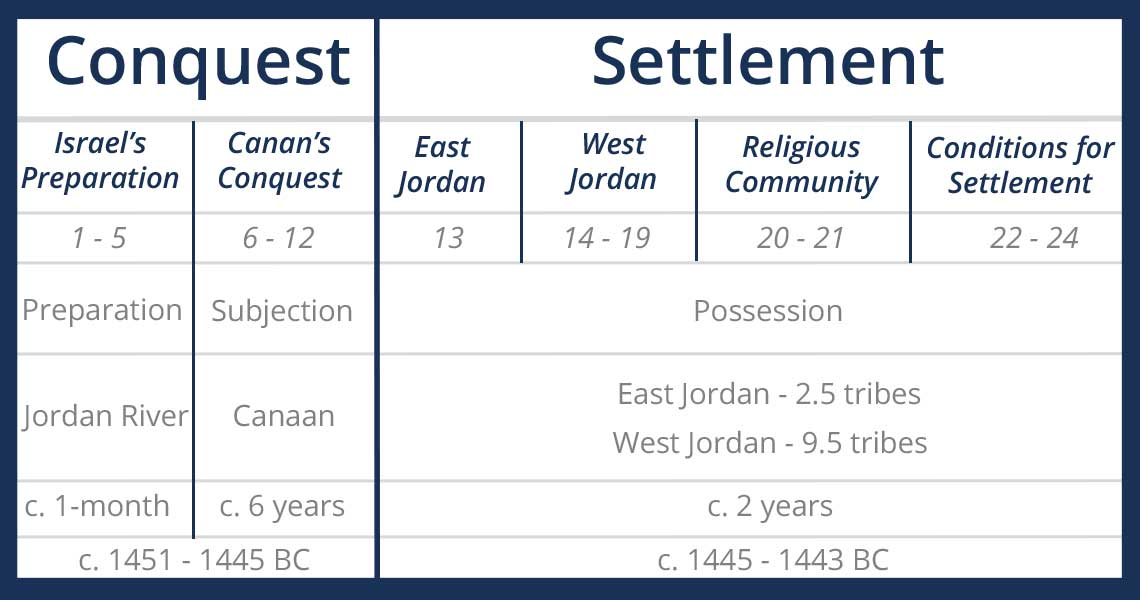
\includegraphics[scale=.5, angle=90]{06OT-Joshua/References/10.Bible-Brief-Joshua.jpg}
\caption[Bible Brief for Joshua]{Bible Brief for Joshua}
\label{fig:Bible Brief for Joshua}
\end{center}
\end{figure}

\newpage
\begin{figure}
\begin{center}
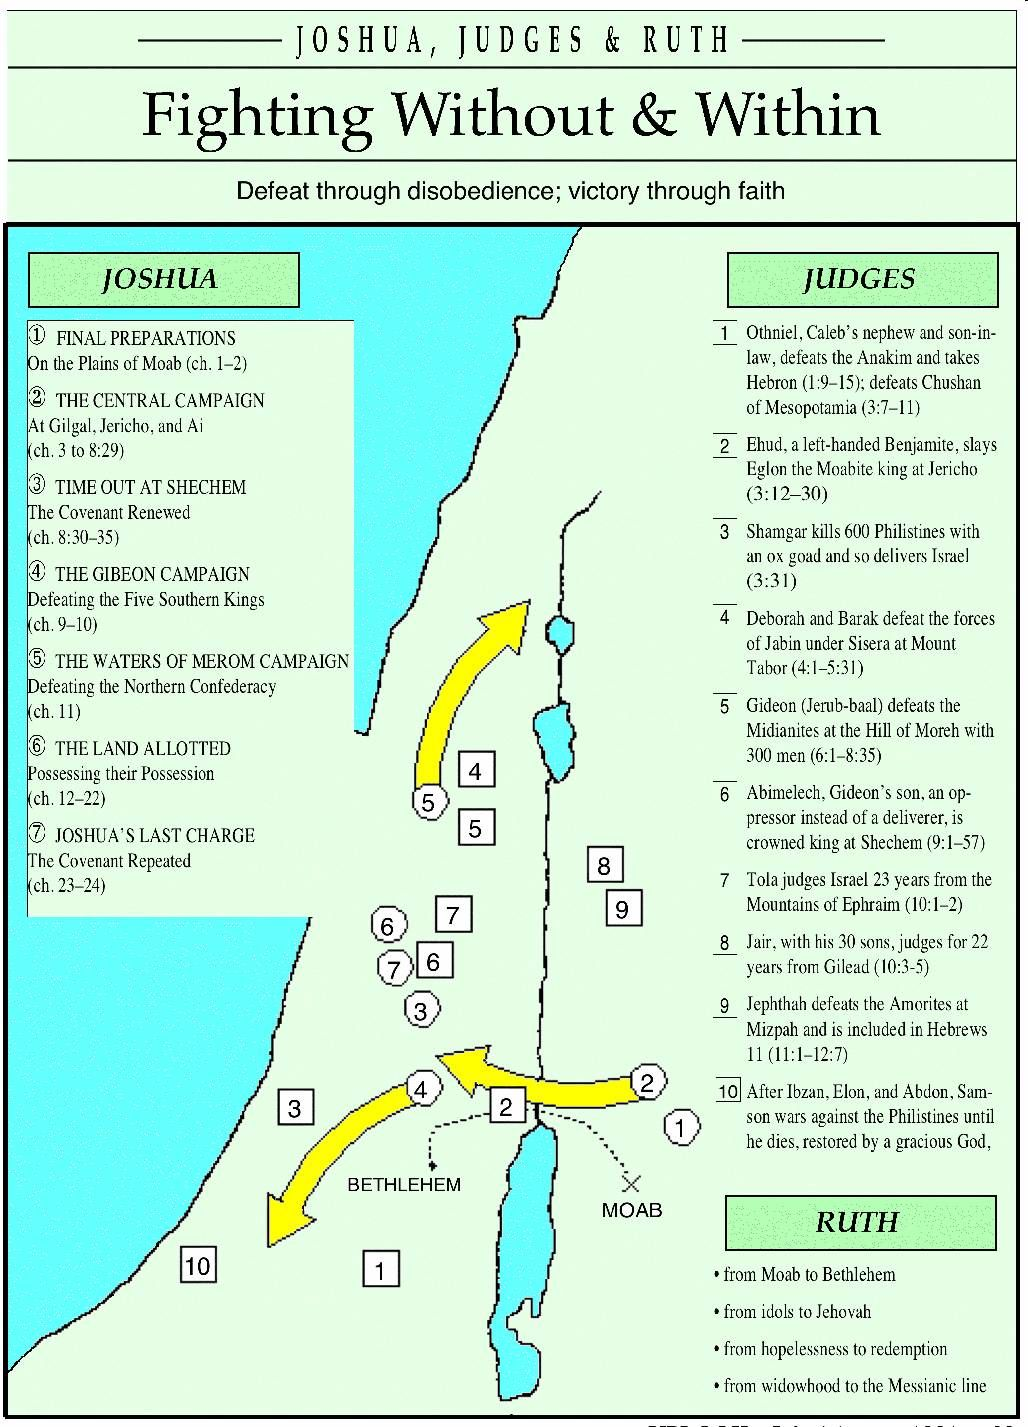
\includegraphics[scale=.5, angle=0]{06OT-Joshua/References/11.FightingInJoshuaAndJudges.jpg}
\caption[The Fighting in Joshua and Judges]{The Fighting in Joshua and Judges}
\label{fig:The Fighting in Joshua and Judges}
\end{center}
\end{figure}

\newpage
\begin{figure}
\begin{center}
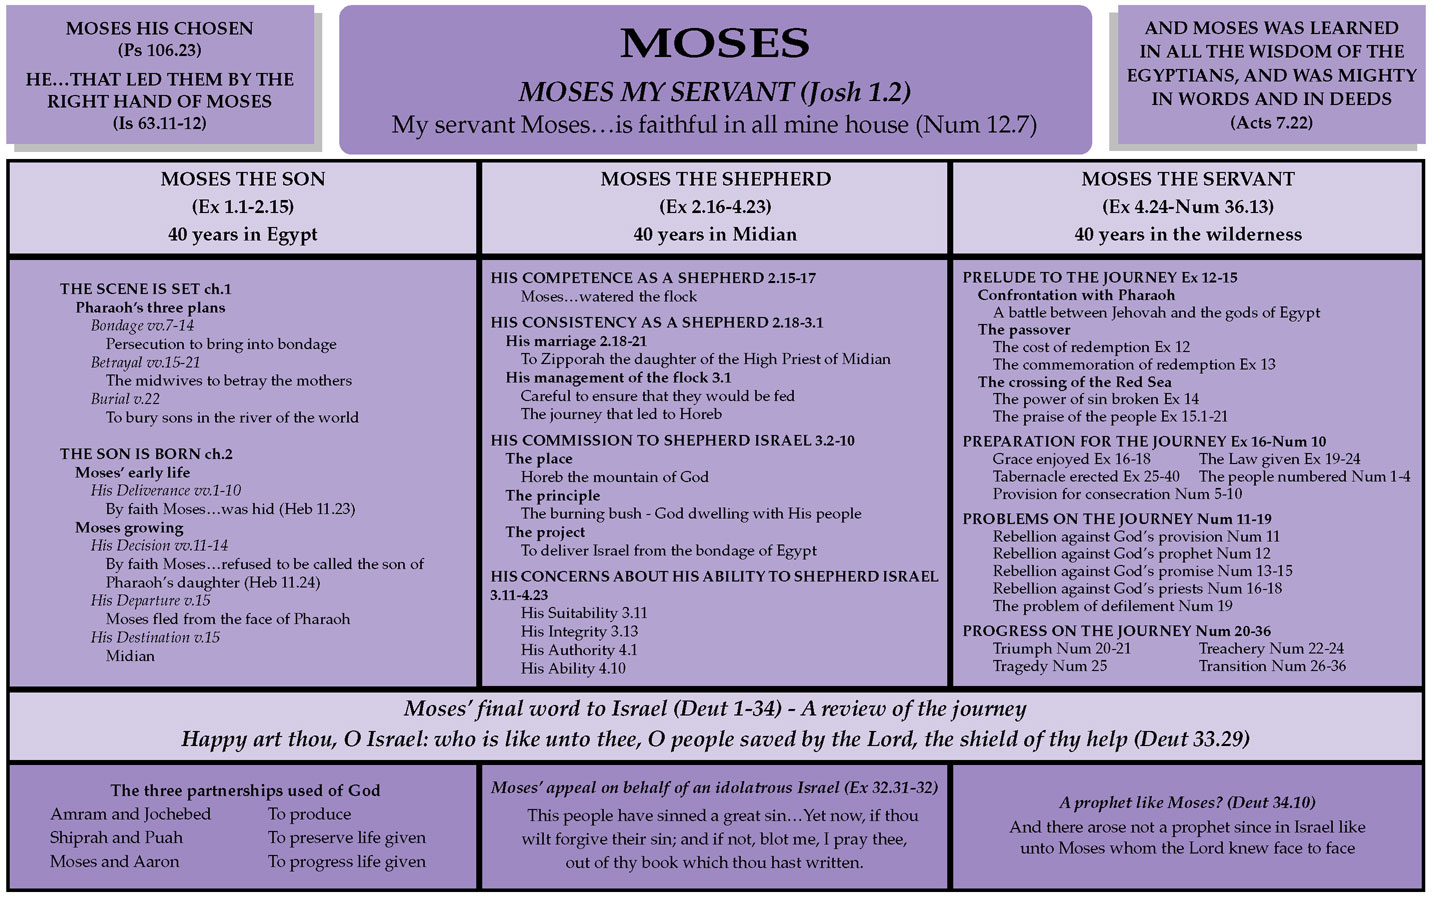
\includegraphics[scale=.4, angle=90]{06OT-Joshua/References/12.JohnGrantMoses.jpg}
\caption[Moses from John Grant]{Moses from John Grant}
\label{fig:Moses from John Grant}
\end{center}
\end{figure}







\chapter{Psalm 1}

\begin{figure}
  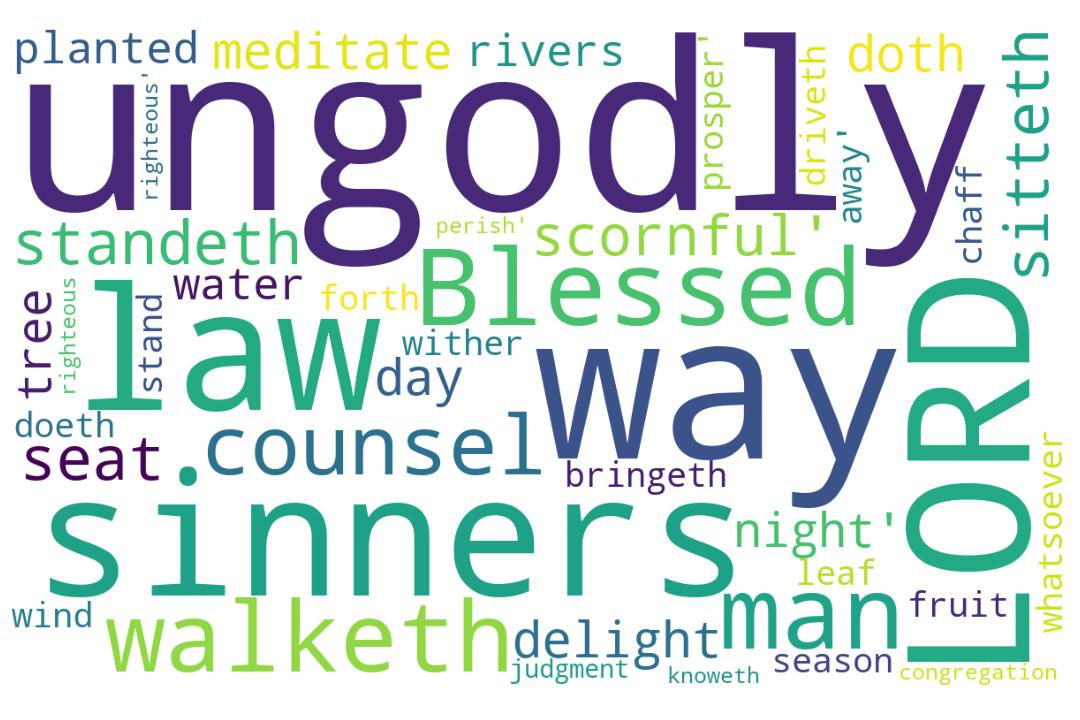
\includegraphics[width=\linewidth]{19OT-Psalms/Psalm1-WordCloud.jpg}
  \caption{Psalm 1 Word Cloud}
  \label{fig:Psalm 1 word Cloud}
\end{figure}


\marginpar{\scriptsize \centering \fcolorbox{bone}{lime}{\textbf{A PSALM OF COMPARISON}}\\ (Psalm 1) 
\begin{compactenum}[I.][8]
    \item A \textbf{Downward Cycle} \index[scripture]{Psalms!Psa 001:01}(Psa 1:1)
    \item A \textbf{Dialobical Counsel} \index[scripture]{Psalms!Psa 001:01}(Psa 1:1)
    \item \textbf{Diligent Consideration} \index[scripture]{Psalms!Psa 001:02}(Psa 1:2)
    \item A \textbf{Different Course} \index[scripture]{Psalms!Psa 001:02}(Psa 1:2)
    \item \textbf{Driven Chaff} \index[scripture]{Psalms!Psa 001:04}(Psa 1:4)
    \item \textbf{Distinguishing Characteristics}  \index[scripture]{Psalms!Psa 001:04}(Psa 1:4)
    \item A \textbf{Delivered Congregation} \index[scripture]{Psalms!Psa 001:05}(Psa 1:5)
    \item A \textbf{Definite Conclusion} \index[scripture]{Psalms!Psa 001:06}(Psa 1:6)
\end{compactenum} }

\marginpar{\scriptsize \centering \fcolorbox{bone}{yellow}{\textbf{THE PSALM 1 MAN}}\\ (Psalm 1) 
\begin{compactenum}[I.][8]
    \item \textbf{Shuns Fools} \index[scripture]{Psalms!Psa 001:01}(Psa 1:1)
    \item Has \textbf{Select Friends} \index[scripture]{Psalms!Psa 001:01}(Psa 1:1)
    \item Eats \textbf{Spiritual Food} \index[scripture]{Psalms!Psa 001:02}(Psa 1:2)
    \item Has \textbf{Special Fellowship} \index[scripture]{Psalms!Psa 001:02}(Psa 1:2)
    \item Exercises \textbf{Simple Faith} (All)
    \item Has his \textbf{Sins Forgiven} (All)
    \item He Can \textbf{Sense Falsehood}
    \item He \textbf{Sees the Future}
    \item Has a \textbf{Spectacular \& Secure Finish} \index[scripture]{Psalms!Psa 001:06}(Psa 1:6)
\end{compactenum}}



\marginpar{\scriptsize \centering \fcolorbox{bone}{black}{\textcolor{white}{\textbf{A COSMIC COMPARISON}}}\\ (Psalm 1) 
\begin{compactenum}[I.]
    \item They have Different \textbf{Objectives}
    \item They have Different \textbf{Orientations}
    \item They have Different \textbf{Obsessions}
    \item They have Different \textbf{Orientations}
    \item They have Different \textbf{Obstacles}
    \item They have Different \textbf{Outcomes}
\end{compactenum}}


\marginpar{\scriptsize \centering \fcolorbox{bone}{blue}{\textcolor{white}{\textbf{ON THE ROAD TO SCORN}}}\\ (Psalm 1) 
\begin{compactenum}[I.]
    \item Not \textbf{Recognizing Blessings}
    \item \textbf{Reviling the Brethren}
    \item Not \textbf{Reading the Book}
    \item \textbf{Revelling in Bitterness}
    \item Not \textbf{Remembering the Burdens}
    \item Not \textbf{Regarding the Body}
    \item Not Carrying the \textbf{Burdens of Believers}
\end{compactenum} }

\marginpar{\scriptsize \centering \fcolorbox{bone}{orange}{\textbf{THE UNGODLY}}\\ (Psalm 1) 

\begin{compactenum}[I.][8]
	\item ungodly \textbf{man} \index[scripture]{Psalms!Psa 001:01}  \index[scripture]{Psalms!Psa 001:04}  \index[scripture]{Psalms!Psa 001:05}  \index[scripture]{Psalms!Psa 003:07}  \index[scripture]{Psalms!Psa 018:04}  \index[scripture]{Proverbs!Pro 16:27} \index[scripture]{Romans!Rom 04:04} (Psa 1:1, 1:4, 1:5, 3:7, 18:4, Pro 16:27, Rom 4:4)
	\item ungoldy \textbf{men} \index[scripture]{2 Samuel!2Sam 22:05} \index[scripture]{2 Chronicles!2Chr 19:02} (2Sam 22:5, 2Chr 19:2, Job 16:11, Job 34:18, Psa 1:6, Psa 73:12, 1Tim 1:9, 1Pet 4:18, 2Pet 2:5, 2Pet 2:6, 2Pet 2:7, Jude 1:4, Jude 1:15)
	  \index[scripture]{Job!Job 16:11}\index[scripture]{Job!Job 34:18} \index[scripture]{Psalms!Psa 001:06} \index[scripture]{Psalms!Psa 073:12}\index[scripture]{1 Timothy!1Tim 01:09} \index[scripture]{1 Peter!1Pet 04:18}\index[scripture]{2 Peter!2Pet 02:05}\index[scripture]{2 Peter!2Pet 02:06}\index[scripture]{2 Peter!2Pet 02:07}\index[scripture]{Jude!Jude 01:15}
	\item ungodly \textbf{nation} \index[scripture]{Psalms!Psa 043:01} (Psa 43:1)
	\item ungodly \textbf{witness} \index[scripture]{Proverbs!Pro 19:28} (Pro 19:28)
	\item ungodly \textbf{deeds} \index[scripture]{Jude!Jude 01:15} (Jude 1:15)
	\item ungodly \textbf{actions} \index[scripture]{Jude!Jude 01:15} (Jude 1:15)
	\item ungodly \textbf{lusts} \index[scripture]{Jude!Jude 01:18} (Jude 1:18)
\end{compactenum}}



\footnote{\textcolor[cmyk]{0.99998,1,0,0}{\hyperlink{TOC}{Return to end of Table of Contents.}}}\footnote{\href{https://www.audioverse.org/english/audiobibles/books/ENGKJV/O/Ps/1}{\textcolor[cmyk]{0.99998,1,0,0}{Psalms Audio}}}\textcolor[cmyk]{0.99998,1,0,0}{Blessed is the man that \fcolorbox{bone}{lime}{walketh} not in the counsel of the \fcolorbox{bone}{lime}{ungodly}, nor \fcolorbox{bone}{lime}{standeth} in the way of sinners, nor \fcolorbox{bone}{lime}{sitteth} in the seat of the scornful.}
[2] \textcolor[cmyk]{0.99998,1,0,0}{But\textcolor{jungle}{$_{29}$} his delight is in the \fcolorbox{bone}{lime}{law of the LORD}; and in his law doth he meditate \fcolorbox{bone}{lime}{day and night}.}
[3] \textcolor[cmyk]{0.99998,1,0,0}{And\textcolor{jungle}{$_{49}$} he shall be like a tree planted by the rivers of water, that bringeth forth his fruit in his season; his leaf also shall not wither; and whatsoever he doeth shall prosper.}\footnote{\textbf{Jeremiah 17:8} -- For he shall be as a tree planted by the waters, and \emph{that} spreadeth out her roots by the river, and shall not see when heat cometh, but her leaf shall be green; and shall not be careful in the year of drought, neither shall cease from yielding fruit.}\footnote{The phrase ``rivers of water'' is found here in Psalm 1:3, Proverbs 21:1, Isaiah 32:2, and Lamentations 3:48. Interestingly, Isaiah 32:2 sets it in a Millennial context.}
[4] \textcolor[cmyk]{0.99998,1,0,0}{The\textcolor{jungle}{$_{82}$} ungodly are not so: but are \fcolorbox{bone}{lime}{like} the \fcolorbox{bone}{lime}{chaff} which the wind driveth away.}\footnote{The word ``chaff'' is found 14 times in 14 verses in scripture, only twice in the New Testament (Mathew 3:12 and Luke 3:17) speaking of the chaff which will be burnt up with unquenchable fire. See: (1) Job 21:18, (2)  Psalm 1:4 (here),  (3) Psalm 35:5, (4)  Isaiah 5:24, (5)  Isaiah 17:13, (6)  Isaiah 29:5, (7) Isaiah 33:11, (8)  Isaiah 41:15, (9) Jeremiah 23:28, (10) Daniel 2:35, (11) Hosea 13:3, (12) Zephaniah 2:2, (13) Matthew 3:12, and (14) Luke 3:17.} 
[5] \textcolor[cmyk]{0.99998,1,0,0}{Therefore\textcolor{jungle}{$_{113}$} the ungodly shall not stand in the judgment, nor sinners in the \fcolorbox{bone}{lime}{congregation} of the righteous.}
[6] \textcolor[cmyk]{0.99998,1,0,0}{For\textcolor{jungle}{$_{114}$} the LORD knoweth the way of the righteous: but the way of the ungodly \fcolorbox{bone}{lime}{shall perish}\textcolor{jungle}{$_{130}$}.}\footnote{\textbf{Psalm 49:12, 17--20} -- Nevertheless man being in honour abideth not: he is like the beasts that perish. [17]  For when he dieth he shall carry nothing away: his glory shall not descend after him.  [18]  Though while he lived he blessed his soul: and men will praise thee, when thou doest well to thyself. [19]  He shall go to the generation of his fathers; they shall never see light.  [20]  Man that is in honour, and understandeth not, is like the beasts that perish.}


\section{Psalm 1 Comments}

\subsection{Numeric Nuggets}
\textbf{13:} Verses 4 and 5 have 13 unique words.\\
\noindent \textbf{66:} There are 66 unique words in Psalm 1.

\subsection{Psalm 1 Introduction}
Note, there are (at least) seven distinct things spoken of in the psalm:
\begin{compactenum}
    \item The counsel of the ungodly [1]
    \item The way of sinners (equated with the way of the ungodly in verse 6) [1]
    \item The seat of the scornful [1]
    \item The Law of the LORD [2]
    \item A Tree planted by the rivers of water [3]
    \item The judgment [5]
    \item The congregation of the righteous [6]
\end{compactenum}


\subsection{Psalm 1:1}
Compare this to the opposite progression in Deuteronomy 5:1: Hear, learn, keep, and do.
%\index[NWIV]{28!Psalms!Psa 1:1}\index[AWIP]{Blessed!Psalms!Psa 1:1}\index[AWIP]{is!Psalms!Psa 1:1}\index[AWIP]{the!Psalms!Psa 1:1}\index[AWIP]{the!Psalms!Psa 1:1 (2)}\index[AWIP]{the!Psalms!Psa 1:1 (3)}\index[AWIP]{the!Psalms!Psa 1:1 (4)}\index[AWIP]{the!Psalms!Psa 1:1 (5)}\index[AWIP]{the!Psalms!Psa 1:1 (6)}\index[AWIP]{man!Psalms!Psa 1:1}\index[AWIP]{that!Psalms!Psa 1:1}\index[AWIP]{walketh!Psalms!Psa 1:1}\index[AWIP]{not!Psalms!Psa 1:1}\index[AWIP]{in!Psalms!Psa 1:1}\index[AWIP]{in!Psalms!Psa 1:1 (2)}\index[AWIP]{in!Psalms!Psa 1:1 (3)}\index[AWIP]{counsel!Psalms!Psa 1:1}\index[AWIP]{of!Psalms!Psa 1:1}\index[AWIP]{of!Psalms!Psa 1:1 (2)}\index[AWIP]{of!Psalms!Psa 1:1 (3)}\index[AWIP]{ungodly!Psalms!Psa 1:1}\index[AWIP]{nor!Psalms!Psa 1:1}\index[AWIP]{nor!Psalms!Psa 1:1 (2)}\index[AWIP]{standeth!Psalms!Psa 1:1}\index[AWIP]{way!Psalms!Psa 1:1}\index[AWIP]{sinners!Psalms!Psa 1:1}\index[AWIP]{sitteth!Psalms!Psa 1:1}\index[AWIP]{seat!Psalms!Psa 1:1}\index[AWIP]{scornful!Psalms!Psa 1:1}

\index[NWIV]{20!Psalms!Psa 1:2}\index[AWIP]{But!Psalms!Psa 1:2}\index[AWIP]{his!Psalms!Psa 1:2}\index[AWIP]{his!Psalms!Psa 1:2 (2)}\index[AWIP]{delight!Psalms!Psa 1:2}\index[AWIP]{is!Psalms!Psa 1:2}\index[AWIP]{in!Psalms!Psa 1:2}\index[AWIP]{in!Psalms!Psa 1:2 (2)}\index[AWIP]{the!Psalms!Psa 1:2}\index[AWIP]{the!Psalms!Psa 1:2 (2)}\index[AWIP]{law!Psalms!Psa 1:2}\index[AWIP]{law!Psalms!Psa 1:2 (2)}\index[AWIP]{of!Psalms!Psa 1:2}\index[AWIP]{LORD!Psalms!Psa 1:2}\index[AWIP]{and!Psalms!Psa 1:2}\index[AWIP]{and!Psalms!Psa 1:2 (2)}\index[AWIP]{doth!Psalms!Psa 1:2}\index[AWIP]{he!Psalms!Psa 1:2}\index[AWIP]{meditate!Psalms!Psa 1:2}\index[AWIP]{day!Psalms!Psa 1:2}\index[AWIP]{night!Psalms!Psa 1:2}

\index[NWIV]{33!Psalms!Psa 1:3}\index[AWIP]{And!Psalms!Psa 1:3}\index[AWIP]{he!Psalms!Psa 1:3}\index[AWIP]{he!Psalms!Psa 1:3 (2)}\index[AWIP]{shall!Psalms!Psa 1:3}\index[AWIP]{shall!Psalms!Psa 1:3 (2)}\index[AWIP]{shall!Psalms!Psa 1:3 (3)}\index[AWIP]{be!Psalms!Psa 1:3}\index[AWIP]{like!Psalms!Psa 1:3}\index[AWIP]{a!Psalms!Psa 1:3}\index[AWIP]{tree!Psalms!Psa 1:3}\index[AWIP]{planted!Psalms!Psa 1:3}\index[AWIP]{by!Psalms!Psa 1:3}\index[AWIP]{the!Psalms!Psa 1:3}\index[AWIP]{rivers!Psalms!Psa 1:3}\index[AWIP]{of!Psalms!Psa 1:3}\index[AWIP]{water!Psalms!Psa 1:3}\index[AWIP]{that!Psalms!Psa 1:3}\index[AWIP]{bringeth!Psalms!Psa 1:3}\index[AWIP]{forth!Psalms!Psa 1:3}\index[AWIP]{his!Psalms!Psa 1:3}\index[AWIP]{his!Psalms!Psa 1:3 (2)}\index[AWIP]{his!Psalms!Psa 1:3 (3)}\index[AWIP]{fruit!Psalms!Psa 1:3}\index[AWIP]{in!Psalms!Psa 1:3}\index[AWIP]{season!Psalms!Psa 1:3}\index[AWIP]{leaf!Psalms!Psa 1:3}\index[AWIP]{also!Psalms!Psa 1:3}\index[AWIP]{not!Psalms!Psa 1:3}\index[AWIP]{wither!Psalms!Psa 1:3}\index[AWIP]{and!Psalms!Psa 1:3}\index[AWIP]{whatsoever!Psalms!Psa 1:3}\index[AWIP]{doeth!Psalms!Psa 1:3}\index[AWIP]{prosper!Psalms!Psa 1:3}

\index[NWIV]{15!Psalms!Psa 1:4}\index[AWIP]{The!Psalms!Psa 1:4}\index[AWIP]{ungodly!Psalms!Psa 1:4}\index[AWIP]{are!Psalms!Psa 1:4}\index[AWIP]{are!Psalms!Psa 1:4 (2)}\index[AWIP]{not!Psalms!Psa 1:4}\index[AWIP]{so!Psalms!Psa 1:4}\index[AWIP]{but!Psalms!Psa 1:4}\index[AWIP]{like!Psalms!Psa 1:4}\index[AWIP]{the!Psalms!Psa 1:4}\index[AWIP]{the!Psalms!Psa 1:4 (2)}\index[AWIP]{chaff!Psalms!Psa 1:4}\index[AWIP]{which!Psalms!Psa 1:4}\index[AWIP]{wind!Psalms!Psa 1:4}\index[AWIP]{driveth!Psalms!Psa 1:4}\index[AWIP]{away!Psalms!Psa 1:4}

\index[NWIV]{17!Psalms!Psa 1:5}\index[AWIP]{Therefore!Psalms!Psa 1:5}\index[AWIP]{the!Psalms!Psa 1:5}\index[AWIP]{the!Psalms!Psa 1:5 (2)}\index[AWIP]{the!Psalms!Psa 1:5 (3)}\index[AWIP]{the!Psalms!Psa 1:5 (4)}\index[AWIP]{ungodly!Psalms!Psa 1:5}\index[AWIP]{shall!Psalms!Psa 1:5}\index[AWIP]{not!Psalms!Psa 1:5}\index[AWIP]{stand!Psalms!Psa 1:5}\index[AWIP]{in!Psalms!Psa 1:5}\index[AWIP]{in!Psalms!Psa 1:5 (2)}\index[AWIP]{judgment!Psalms!Psa 1:5}\index[AWIP]{nor!Psalms!Psa 1:5}\index[AWIP]{sinners!Psalms!Psa 1:5}\index[AWIP]{congregation!Psalms!Psa 1:5}\index[AWIP]{of!Psalms!Psa 1:5}\index[AWIP]{righteous!Psalms!Psa 1:5}

\index[NWIV]{17!Psalms!Psa 1:6}\index[AWIP]{For!Psalms!Psa 1:6}\index[AWIP]{the!Psalms!Psa 1:6}\index[AWIP]{the!Psalms!Psa 1:6 (2)}\index[AWIP]{the!Psalms!Psa 1:6 (3)}\index[AWIP]{the!Psalms!Psa 1:6 (4)}\index[AWIP]{the!Psalms!Psa 1:6 (5)}\index[AWIP]{LORD!Psalms!Psa 1:6}\index[AWIP]{knoweth!Psalms!Psa 1:6}\index[AWIP]{way!Psalms!Psa 1:6}\index[AWIP]{way!Psalms!Psa 1:6 (2)}\index[AWIP]{of!Psalms!Psa 1:6}\index[AWIP]{of!Psalms!Psa 1:6 (2)}\index[AWIP]{righteous!Psalms!Psa 1:6}\index[AWIP]{but!Psalms!Psa 1:6}\index[AWIP]{ungodly!Psalms!Psa 1:6}\index[AWIP]{shall!Psalms!Psa 1:6}\index[AWIP]{perish!Psalms!Psa 1:6}


\section{Psalm 1 Outlines}

\subsection{My Outlines}

\subsubsection{A Psalm of Comparisons}
\textbf{Introduction: }Psalm 1 compares the path of the righteous and the paths of the ungodly:
\index[speaker]{Keith Anthony!Psalm 001 (A Psalm of Comparisons)}
\index[series]{Psalms (Keith Anthony)!Psalm 001 (A Psalm of Comparisons)}
\index[date]{2015/08/24!Psalm 001 (A Psalm of Comparisons) (Keith Anthony)}
\begin{compactenum}[I.]
    \item A \textbf{Downward Cycle} \index[scripture]{Psalms!Psa 001:01}(Psa 1:1)
    \item A \textbf{Dialobical Counsel} \index[scripture]{Psalms!Psa 001:01}(Psa 1:1)
    \item \textbf{Diligent Consideration} \index[scripture]{Psalms!Psa 001:02}(Psa 1:2)
    \item A \textbf{Different Course} \index[scripture]{Psalms!Psa 001:02}(Psa 1:2)
    \item \textbf{Driven Chaff} \index[scripture]{Psalms!Psa 001:04}(Psa 1:4)
    \item \textbf{Distinguishing Characteristics}  \index[scripture]{Psalms!Psa 001:04}(Psa 1:4)
    \item A \textbf{Delivered Congregation} \index[scripture]{Psalms!Psa 001:05}(Psa 1:5)
    \item A \textbf{Definite Conclusion} \index[scripture]{Psalms!Psa 001:06}(Psa 1:6)
\end{compactenum}

\subsubsection{The Psalm 1 Man}
Psalm 1 provides a description of a different sort of man.  The man seeks God.  He seeks truth and righteousness.  He is radically different from the man of the world, and the man of the flesh, and the man who seeks the Devil. The Psalm 1 man: %\footnote{05 June 2015, Prepared for Lebanon Baptist Temple preaching class}
\index[speaker]{Keith Anthony!Psalm 001 (The Psalm 1 Man)}
\index[series]{Psalms (Keith Anthony)!Psalm 001 (The Psalm 1 Man)}
\index[date]{2015/06/05!Psalm 001 (The Psalm 1 Man) (Keith Anthony)}


\index[LOCATION]{Greene County Adult Detention Center!2022/01/11!Tuesday Night}

\begin{compactenum}[I.]
    \item \fcolorbox{bone}{yellow}{\textbf{Shuns Fools}} \index[scripture]{Psalms!Psa 001:01}(Psa 1:1) The word fool is used 66 times in the King James. The word ``fools'' is found another 42 times. ``Foolish'' is found 52 times! Foolishly, 12 times; foolishness, 20 times. That's 199 times that variants of the word are found (78 times in Proverbs).How about:
    \begin{compactenum}[A.]
		\item Psalm 14:1: The fool hath said in his heart, There is no God. They are corrupt, they have done abominable works, there is none that doeth good.
		\item Psalm 74:18:O LORD, and that the foolish people have blasphemed thy name.
		\item Proverb 27:3:  Though thou shouldest bray a fool in a mortar among wheat with a pestle, yet will not his foolishness depart from him. (stuck on folly)
	\end{compactenum}
    \item \fcolorbox{bone}{yellow}{Has \textbf{Select Friends}} \index[scripture]{Psalms!Psa 001:01}(Psa 1:1)
    \begin{compactenum}[A.]
    	\item 1 Corinthians 15:33 Be not deceived: evil communications corrupt good manners.
    	\item Proverb 12;26 The righteous is more excellent than his neighbour: but the way of the wicked seduceth them.
    	\item Proverb 13:20 He that walketh with wise men shall be wise: but a companion of fools shall be destroyed.
    	\item Proverb 20:19 He that goeth about as a talebearer revealeth secrets: therefore meddle not with him that flattereth with his lips.
    	\item Proverb 22:24-25 Make no friendship with an angry man; and with a furious man thou shalt not go: 25 Lest thou learn his ways, and get a snare to thy soul.
    	\item Proverb 24:6 For by wise counsel thou shalt make thy war: and in multitude of counsellors there is safety.
    	\item 2 Corinthians 6:14 Be ye not unequally yoked together with unbelievers: for what fellowship hath righteousness with unrighteousness? and what communion hath light with darkness?
    \end{compactenum}
	\item \fcolorbox{bone}{yellow}{Eats \textbf{Spiritual Food}} \index[scripture]{Psalms!Psa 001:02}(Psa 1:2) - Spiritual food is the blessings of God. It is typified by manna in the Old testament. Obedience is spiritual food. Doctrine is spiritual food. Worship is spiritual food. Prayer is spiritual food. Some verses:
    \begin{compactenum}[A.]
		\item 1 Corinthians 10:1-4 Moreover, brethren, I would not that ye should be ignorant, how that all our fathers were under the cloud, and all passed through the sea; 2 And were all baptized unto Moses in the cloud and in the sea; 3 And did all eat the same spiritual meat; 4 And did all drink the same spiritual drink: for they drank of that spiritual Rock that followed them: and that Rock was Christ.
		\item 1 Peter 2:2 As newborn babes, desire the sincere milk of the word, that ye may grow thereby:
		\item Hebrews 5:12-14 For when for the time ye ought to be teachers, ye have need that one teach you again which be the first principles of the oracles of God; and are become such as have need of milk, and not of strong meat. 13 For every one that useth milk is unskilful in the word of righteousness: for he is a babe. 14 But strong meat belongeth to them that are of full age, even those who by reason of use have their senses exercised to discern both good and evil.
		\item Jeremiah 3:15 And I will give you pastors according to mine heart, which shall feed you with knowledge and understanding.
		\item John 6:51 I am the living bread which came down from heaven: if any man eat of this bread, he shall live for ever: and the bread that I will give is my flesh, which I will give for the life of the world.
		\item Revealtion 2:7 He that hath an ear, let him hear what the Spirit saith unto the churches; To him that overcometh will I give to eat of the tree of life, which is in the midst of the paradise of God.
    \end{compactenum}
    \item \fcolorbox{bone}{yellow}{Has \textbf{Special Fellowship}} \index[scripture]{Psalms!Psa 001:02}(Psa 1:2) with God and with believers and with scripture
    \begin{compactenum}[A.]
    	\item Colossians 3:16 Let the word of Christ dwell in you richly in all wisdom; teaching and admonishing one another in psalms and hymns and spiritual songs, singing with grace in your hearts to the Lord.
		\item Romans 1:12 That is, that I may be comforted together with you by the mutual faith both of you and me.
		\item Hebrews 10:24-25 And let us consider one another to provoke unto love and to good works: 25 Not forsaking the assembling of ourselves together, as the manner of some is; but exhorting one another: and so much the more, as ye see the day approaching.
    \end{compactenum}
    \item \fcolorbox{bone}{yellow}{He Can \textbf{Sense Falsehood(s)} }
        \begin{compactenum}[A.]
        	\item 1 Chronicles 12:32 And of the children of Issachar, which were men that had understanding of the times, to know what Israel ought to do; the heads of them were two hundred; and all their brethren were at their commandment.
        	\item Psalm 119:105 Thy word is a lamp unto my feet, and a light unto my path.
        	\item Hebrews 5:15 But strong meat belongeth to them that are of full age, even those who by reason of use have their senses exercised to discern both good and evil.
           \end{compactenum}
     \item \fcolorbox{bone}{yellow}{He \textbf{Sees the Future}} Bible, carefully studied and rightly divided, records the essential human history and clearly lays out the future
    \begin{compactenum}[A.]
    	\item Amos 3:7 Surely the Lord GOD will do nothing, but he revealeth his secret unto his servants the prophets.
    	\item Acts 1:7-8 And he said unto them, It is not for you to know the times or the seasons, which the Father hath put in his own power. 8 But ye shall receive power, after that the Holy Ghost is come upon you: and ye shall be witnesses unto me both in Jerusalem, and in all Judæa, and in Samaria, and unto the uttermost part of the earth.
    \end{compactenum}
    \item \fcolorbox{bone}{yellow}{Has his \textbf{Sins Forgiven}} (All)
    \begin{compactenum}[A.]
    	\item Isaiah 1:18  Come now, and let us reason together, saith the LORD: though your sins be as scarlet, they shall be as white as snow; though they be red like crimson, they shall be as wool.
    	\item Isaiah 55:7  Let the wicked forsake his way, and the unrighteous man his thoughts: and let him return unto the LORD, and he will have mercy upon him; and to our God, for he will abundantly pardon.
    	\item John 3:1-17 For God so loved the world, that he gave his only begotten Son, that whosoever believeth in him should not perish, but have everlasting life. 17 For God sent not his Son into the world to condemn the world; but that the world through him might be saved.
    	\item Romans 6:23 For the wages of sin is death; but the gift of God is eternal life through Jesus Christ our Lord.
    	\item Romans 8:1 There is therefore now no condemnation to them which are in Christ Jesus, who walk not after the flesh, but after the Spirit.
		\item 1 John 1:9 If we confess our sins, he is faithful and just to forgive us our sins, and to cleanse us from all unrighteousness.
		\item 1 John 2:12 I write unto you, little children, because your sins are forgiven you for his name’s sake.
    \end{compactenum}
    \item \fcolorbox{bone}{yellow}{Has a \textbf{Spectacular \& Secure Finish}} \index[scripture]{Psalms!Psa 001:06}(Psa 1:6)
    \begin{compactenum}[A.]
		\item John 3:14-16 And as Moses lifted up the serpent in the wilderness, even so must the Son of man be lifted up: 15 That whosoever believeth in him should not perish, but have eternal life.
16 ¶ For God so loved the world, that he gave his only begotten Son, that whosoever believeth in him should not perish, but have everlasting life.
		\item Romans 6:23 For the wages of sin is death; but the gift of God is eternal life through Jesus Christ our Lord.
		\item John 4:14  But whosoever drinketh of the water that I shall give him shall never thirst; but the water that I shall give him shall be in him a well of water springing up into everlasting life.
		\item 1 John 2:25 And this is the promise that he hath promised us, even eternal life.
		\item Titus 3:3-7 For we ourselves also were sometimes foolish, disobedient, deceived, serving divers lusts and pleasures, living in malice and envy, hateful, and hating one another. 4 But after that the kindness and love of God our Saviour toward man appeared, 5 Not by works of righteousness which we have done, but according to his mercy he saved us, by the washing of regeneration, and renewing of the Holy Ghost; 6 Which he shed on us abundantly through Jesus Christ our Saviour; 7 That being justified by his grace, we should be made heirs according to the hope of eternal life. 
    \end{compactenum}
    \item Exercises \textbf{Simple Faith} (All)
    \begin{compactenum}[A.]
		\item Matthew 18:3 And said, Verily I say unto you, Except ye be converted, and become as little children, ye shall not enter into the kingdom of heaven
		\item Luke 18:17 Verily I say unto you, Whosoever shall not receive the kingdom of God as a little child shall in no wise enter therein
		\item Hebrews 11:6 ut without faith it is impossible to please him: for he that cometh to God must believe that he is, and that he is a rewarder of them that diligently seek him.
		\item Romans 10:17  So then faith cometh by hearing, and hearing by the word of God.
		\item Romans 1:17  For therein is the righteousness of God revealed from faith to faith: as it is written, The just shall live by faith.
    \end{compactenum}
\end{compactenum}

\subsubsection{A Cosmic Comparison}
Psalm 1 contrasts an ungodly man with one who seeks God Almighty. There are numerous differences.  Among them: %\footnote{04 June 2015, Prepared for Lebanon Baptist Temple preaching class}
\index[speaker]{Keith Anthony!Psalm 001 (A Cosmic Comparison)}
\index[series]{Psalms (Keith Anthony)!Psalm 001 (A Cosmic Comparison)}
\index[date]{2015/06/04!Psalm 001 (A Cosmic Comparison) (Keith Anthony)}
\begin{compactenum}[I.]
    \item They have Different \textbf{Objectives}
    \item They have Different \textbf{Orientations}
    \item They have Different \textbf{Obsessions}
    \item They have Different \textbf{Orientations}
    \item They have Different \textbf{Obstacles}
    \item They have Different \textbf{Outcomes}
\end{compactenum}

\subsubsection{Road-markers on the Road to Scorn}
I know a little bit about this, as does any Christian who has lived for more than a few years. Psalm 1 talks about the seat of the scornful.  Almost any Christian or every Christian has been abused by other Christians, mistreated by ministers, misunderstood, etc. Almost every Christian has been at one time or another on the wrong side of an apparent double-standard. These  are all dangerous place to be, as the response or rather how one decides to respond will make a world of difference. If you can picture Christianity as a highway, then there is also another parallel road, probably with a slow lane and a high-speed lane. At any point a Christian can exit off the Christian highway and get on this other road, going the opposite direction. Sometimes it is tough to recognize that you've done so. In Psalm 1, the destinations of these two roads are made known.  The place of blessing and the seat of the scornful. So, I got to thinking more about this road to this seat of the scornful.  What does the path look like?  What are the road-markers? This is just case you are seeing some of these road-markers of late.  Maybe you are on this road to the seat of the scornful. Maybe there are a few road signs that will tell you that you are: 
%\footnote{16 June 2015, Prepared for Lebanon Baptist Temple preaching class}
\index[speaker]{Keith Anthony!Psalm 001 (Road-markers on the Road to Scorn)}
\index[series]{Psalms (Keith Anthony)!Psalm 001 (Road-markers on the Road to Scorn)}
\index[date]{2015/06/16!Psalm 001 (Road-markers on the Road to Scorn) (Keith Anthony)}
\begin{compactenum}[I.]
    \item Not \textbf{Recognizing Blessings}
    \item \textbf{Reviling the Brethren}
    \item Not \textbf{Reading the Book}
    \item \textbf{Revelling in Bitterness}
    \item Not \textbf{Remembering the Burdens}
    \item Not \textbf{Regarding the Body}
    \item Not Carrying the \textbf{Burdens of Believers}
\end{compactenum}

\subsubsection{The Ungodly Man}
Psalm 1 provides insight into the ungodly man. The word ``ungodly'' is found 27 times in 24 verses in scripture, notably 4 times in Jude 15. Here is used in the corporate sense, as in ungodly people. Usages of the word: %\footnote{07 June 2016, Keith Anthony}
\index[speaker]{Keith Anthony!Psalm 001 (The Ungodly Man}
\index[series]{Psalms (Keith Anthony)!Psalm 001 (The Ungodly Man}
\index[date]{2016/06/07!Psalm 001 (The Ungodly Man (Keith Anthony)}
\begin{compactenum}[I.][8]
	\item ungodly \textbf{man} \index[scripture]{Psalms!Psa 001:01}  \index[scripture]{Psalms!Psa 001:04}  \index[scripture]{Psalms!Psa 001:05}  \index[scripture]{Psalms!Psa 003:07}  \index[scripture]{Psalms!Psa 018:04}  \index[scripture]{Proverbs!Pro 16:27} \index[scripture]{Romans!Rom 04:04} (Psa 1:1, 1:4, 1:5, 3:7, 18:4, Pro 16:27, Rom 4:4)
	\item ungoldy \textbf{men} \index[scripture]{2 Samuel!2Sam 22:05} \index[scripture]{2 Chronicles!2Chr 19:02} (2Sam 22:5, 2Chr 19:2, Job 16:11, Job 34:18, Psa 1:6, Psa 73:12, 1Tim 1:9, 1Pet 4:18, 2Pet 2:5, 2Pet 2:6, 2Pet 2:7, Jude 1:4, Jude 1:15)
	  \index[scripture]{Job!Job 16:11}\index[scripture]{Job!Job 34:18} \index[scripture]{Psalms!Psa 001:06} \index[scripture]{Psalms!Psa 073:12}\index[scripture]{1 Timothy!1Tim 01:09} \index[scripture]{1 Peter!1Pet 04:18}\index[scripture]{2 Peter!2Pet 02:05}\index[scripture]{2 Peter!2Pet 02:06}\index[scripture]{2 Peter!2Pet 02:07}\index[scripture]{Jude!Jude 01:15}
	\item ungodly \textbf{nation} \index[scripture]{Psalms!Psa 043:01} (Psa 43:1)
	\item ungodly \textbf{witness} \index[scripture]{Proverbs!Pro 19:28} (Pro 19:28)
	\item ungodly \textbf{deeds} \index[scripture]{Jude!Jude 01:15} (Jude 1:15)
	\item ungodly \textbf{actions} \index[scripture]{Jude!Jude 01:15} (Jude 1:15)
	\item ungodly \textbf{lusts} \index[scripture]{Jude!Jude 01:18} (Jude 1:18)
\end{compactenum}


\subsection{Outlines from Others}

\subsubsection{Bible Study as Worship}
Psalm 1 provides insight into the ungodly man. The word ``ungodly'' is found 27 times in 24 verses in scripture, notably 4 times in Jude 15. Here is used in the corporate sense, as in ungodly people. Usages of the word:\footnote{Kevin Cauley}\\ \\
\index[speaker]{Kevin Cauley!Psalm 001 (Bible Study as Worship}
\index[series]{Psalms (Kevin Cauley)!Psalm 001 (Bible Study as Worship}
\index[date]{2002/07/03!Psalm 001 (Bible Study as Worship) (Kevin Cauley)}
\noindent \textbf{Introduction: }A study of worship in the Bible. In this lesson we will look at Bible Study as Worship. Bible Study is worshiping God because we are 1) Reciting God's Will. 2) Respecting and Honoring God's Word. 3) Retaining God's thoughts in our hearts. 4) Retooling our lives in God's image.  Psalm 1:
\begin{compactenum}[1.][9]
	\item This first Psalm is a Psalm of introduction.
	\item It introduces us to the concept of studying God's word with the intention of applying it to life.
	\item A blessing is pronounced upon the one who does not progress in sin.
	\item He doesn't progress in sin because he has a delight in God's word.
	\item He meditates and thinks about God's word day and night.
	\item The beautiful results are that he is like a tree planted by the waters that brings forth fruit.
	\item This Psalm gives us a picture of worshiping God through the study of His word.
	\item Remember our definition of worship, to bend the knee and prostate oneself toward.
	\item How is this the case with Bible study?
\end{compactenum}
\textbf{\\Discussion: }Discussion: Christians worship God when we study His word because we are
\begin{compactenum}[I.][8]
	\item \textbf{Reciting God's Will} 
	\item  \textbf{Respecting and Honoring God's Words} 
	\item  \textbf{Retaining God's Words in Our Heart} 
	\item  \textbf{Retooling Our Lives in God's Image} 
\end{compactenum}

\subsubsection{Characteristics of the Successful Believer}
Psalm 1 provides insight into the ungodly man. The word ``ungodly'' is found 27 times in 24 verses in scripture, notably 4 times in Jude 15. Here is used in the corporate sense, as in ungodly people. Usages of the word: \\ \\
\index[speaker]{sermonnotebook.org!Psalm 001:01-06 (Characteristics of the Successful Believer}
\index[series]{Psalms (sermonnotebook.org)!Psalm 001 (Characteristics of the Successful Believer}
\index[date]{unknown!Psalm 001 (Characteristics of the Successful Believer) (sermonnotebook.org)}
\noindent \textbf{Introduction: }There are many yardsticks by which men measure success. Among them are: wealth, power, position, prestige, etc. These are all indicators of worldly success. However, measuring your spiritual success and your success as a Christian is a little more difficult. Often, there is little tangible, visible evidence, which you can put your hands on to prove you are living a successful Christian life. Generally, success for the believer is more internal that external. What I mean by that is this, the small amount of external evidence we produce is the result of much internal activity in our hearts and lives. That is why it is difficult for God’s children, who live in a materialistic world, to gauge their success in their walk with God. Thankfully Psalm 1 exists. In this worthy doorkeeper to the psalms, we find insight into what makes a believer successful. Tonight, as the plumbline of God’s Word moves alongside you life, see for yourself just how you measure up to God’s standard for successful Christian living. As we move through this Psalm, allow me to share with you The Characteristics Of The Successful Believer.

\begin{compactenum}[I.][8]
	\item The \textbf{Path} of the Successful Believer \index[scripture]{Psalms!Psa 001:01}(Psalm 1:1)
	\begin{compactenum}[A.]
		\item The Successful believer is separated in his walk of life.
		\item The downward progress – Walk, Stand, Sit. (This is the path Lot took – Gen. 19. It eventually led to his total downfall!)
		\item The successful believer realizes that there is a vast difference between himself and the world he was saved out of, and he lives accordingly!
	\end{compactenum}
	\item The \textbf{Pleasure} of the Successful Believer \index[scripture]{Psalms!Psa 001:02}(Psalm 1:2)
	\item The \textbf{Prosperity} of the Successful Believer \index[scripture]{Psalms!Psa 001:03}(Psalm 1:3)
	\begin{compactenum}[A.]
		\item His \textbf{Position} – By the River! Always close to the life giving resources. (ILLUSTRATION. This was meaningful to Israel with her mostly arid conditions.) The tree planted by the river is never dry and wilted, but is green, lush and lovely. (ILLUSTRATION. The believer who lives close to God will never be dry and wilted either. He will be vibrant, lively and productive.) (ILLUSTRATION. Many never know the joy of drawing off Christ daily! As a result, they are spiritually wilted and dead looking.) The droughts of life and the dry seasons never seem to affect the believer who is planted near the river. He is connected to an unfailing source of life and strength.
		\item His \textbf{Prominence} – ILLUSTRATION. A tree. The life of the successful believerstands heads above all those around him. It is easily seen when a man draws from the Lord. (Ill. Men will know when you have been with Jesus – Acts. 4:13)
		\item His \textbf{Permanence} – Planted – Unlike some plants, which live for a season and die out, this tree, has sunk its root deep and has a hidden source of life. (ILLUSTRATION. The value of private prayer and Bible Study.) (ILLUSTRATION. Planted – literally "transplanted." A tree cannot transplant itself, neither can a man transplant himself into the Kingdom of God. It is wholly a work of God’s grace. And, He always plants us in good soil, near the water supply. However, after we are planted, it is our responsibility to draw from the resources, which God has provided.)
		\item His \textbf{Productivity} – "Brings forth fruit" – The successful believer is a blessing to all those around him, because his fruit is plentiful. (ILLUSTRATION. John 7:38) (ILLUSTRATION. Old apple tree in the cow pasture. Man, cows, birds and insects all benefited from the fruit off this old tree.) (ILLUSTRATION. You may never know just who is feeding off your life!)
		\item His \textbf{Predictability} – "In his season" This tree isn’t a freak. Just as there are seasons of fruit bearing, so there are times of rest and growth. As believers, we aren’t to worry over the fruit. That is the Father’s business! When everything else is as it should be, then the fruit will come in its season – John 15:1-5.
		\item His \textbf{Perpetuity} – "leaf shall not fade" – The successful believer is like an evergreen. He is always surrounded by the green of life. (ILLUSTRATION. The trees in the wintertime. The hardwoods and leafy trees are look dead, but the evergreens stand out as islands of life in a sea of deadness. They are unaffected by winter or weather, but they are always the same.) (ILLUSTRATION. our lives should be lives of consistency! We are called on to be a stable, faithful and dependable people – 1 Cor. 15:58) The successful believer is consistent. The curve balls of life are unable to knock him off course. (ILLUSTRATION. Thank the Lord for consistent people!) (ILLUSTRATION. Life lived by this river in unchanging.)
		\item His \textbf{Prosperity} –"Whatsoever he doeth, it shall prosper" – In other words, God will bless the successful believer. His personal life, his family life, his business life, his church life, his spiritual life will all be blessed of the Lord. That isn’t to say that there won’t be stormy seas, but the successful believer will be able to sail them with Jesus until they are calm once again!
	\end{compactenum}
\end{compactenum}


\subsubsection{How to Identify a Blessed Man}
\index[speaker]{Clark Herring!Psalm 001 (How to Identify a Blessed Man}
\index[series]{Psalms (Clark Herring)!Psalm 001 (How to Identify a Blessed Man}
\index[date]{2018/01/10!Psalm 001 (How to Identify a Blessed Man) (Clark Herring)}
\begin{compactenum}[I.][6]
	\item His Decision \index[scripture]{Psalms!Psa 001:01}(Psalm 1:1)
	\begin{compactenum}[A.]
		\item Sprint (walk)
		\item Stand
		\item Seat
	\end{compactenum}	
	\item His Delight \index[scripture]{Psalms!Psa 001:02}(Psalm 1:2)
	\begin{compactenum}[A.]
		\item Law (2a)
		\item Lord (2b)
		\item Length (2c)
	\end{compactenum}	
	\item His Duration \index[scripture]{Psalms!Psa 001:03}(Psalm 1:3)
	\begin{compactenum}[A.]
		\item Fruitful (3a)
		\item Faithful (3b)
		\item Fortune (3c)
	\end{compactenum}	
	\item His Discouragement \index[scripture]{Psalms!Psa 001:04}(Psalm 1:4)
	\begin{compactenum}[A.]
		\item Satan
		\item Self
		\item Scorners
		\item Saints (jealousy)
	\end{compactenum}	
	\item His Destination \index[scripture]{Psalms!Psa 001:05}(Psalm 1:5)
	\begin{compactenum}[A.]
		\item We have a Place
		\item We have a Position
		\item We have a Pardon
	\end{compactenum}	
	\item His Direction \index[scripture]{Psalms!Psa 001:06}(Psalm 1:6)
	\begin{compactenum}[A.]
		\item Christ (6a)
		\item Confidence (6b)
		\item Comparison (6c)
	\end{compactenum}	
\end{compactenum}

\subsubsection{The Blessed Man}
\index[speaker]{Brian Eades!Psalm 01 (The Blessed Man)}
\index[series]{Psalm (Brian Eades)!Psalm 01 (The Blessed Man)}
\index[date]{2018/11/01!Psalm 01 (The Blessed Man) (Brian Eades)}
\textbf{Source}: Facebook, ``Sermon Hints'' group\\
\textbf{Introduction}: The Bible refers to the word "bless" 463 times; the word "curse" (being the antonym) which is mentioned only 183 times. What does it mean to be blessed? There are people on Earth who are blessed yet have no money or even health. Look at Job...His story is one of tragedy, yet he was the most blessed man on the face of the Earth!\\
\\
BLESSINGS-"Blissfully contented, definely or supremely favored, fortunate, that which brings thankfulness and appreciation."\\
\\
1 Timothy 6:6-10 (KJV) But godliness with contentment is great gain. For we brought nothing into this world, and it is certain we can carry nothing out. And having food and raiment let us be therewith content. But they that will be rich fall into temptation and a snare, and into many foolish and hurtful lusts, which drown men in destruction and perdition. For the love of money is the root of all evil: which while some coveted after, they have erred from the faith, and pierced themselves through with many sorrows.
\begin{compactenum}[I.][7]
	\item The \textbf{INTRODUCTION}   (of the entire Psalms) "Blessed"
	\item The \textbf{INDIVIDUALITY}   "is THE man"
	\item The \textbf{INSTRUCTIONS} 
	\begin{compactenum}[A.]
		\item AVOIDS BAD ADVICE
Walking not in the counsel of the ungodly
(backing)
		\item AVOIDS BAD ACTIONS
Standing not in the way of sinners (behavior)
		\item AVOIDS BAD ATTITUDES
Not sitting in the seat of the scornful (berating)
	\end{compactenum}
\item The \textbf{INSPIRATION} 
	\begin{compactenum}[A.]
		\item READING THE SCRIPTURES (comforted)
		\item ROOTED IN THE STREAM (consistent)
		\item REPRODUCTIVE IN THE SOIL (converting)
		\item READY FOR A SUCCESSFUL LIFE
	\end{compactenum}
\end{compactenum}
%\section{Psalm 1 Statistics}

%%%%%%%%%%%%%%%%%%%%%%%%%%%
%%%%%Word Statistics
%%%%%%%%%%%%%%%%%%%%%%%%%%%


\normalsize



\subsection{Chapter Word Statistics}


%%%%%%%%%%
%%%%%%%%%%
 
\begin{center}
\begin{longtable}{l|c|c|c|c}
\caption[Stats for Psalm 1]{Stats for Psalm 1} \label{table:Stats for Psalm 1} \\ 
\hline \multicolumn{1}{|c|}{\textbf{Verse(s)}} & \multicolumn{1}{|c|}{\textbf{Count}} & \multicolumn{1}{|c|}{\textbf{Unique}} & \multicolumn{1}{|c|}{\textbf{Italics}} & \multicolumn{1}{|c|}{\textbf{Uniq Italic}}  \\ \hline 
\endfirsthead
 
\multicolumn{5}{c}
{{\bfseries \tablename\ \thetable{} -- continued from previous page}} \\  
\hline \multicolumn{1}{|c|}{\textbf{Verse(s)}} & \multicolumn{1}{|c|}{\textbf{Count}} & \multicolumn{1}{|c|}{\textbf{Unique}} & \multicolumn{1}{|c|}{\textbf{Italics}} & \multicolumn{1}{|c|}{\textbf{Uniq Italic}}  \\ \hline 
\endhead
 
\hline \multicolumn{5}{|r|}{{Continued if needed}} \\ \hline
\endfoot 
1 & 28 & 18 & 0 & 0\\ \hline
2 & 20 & 15 & 0 & 0\\ \hline
3 & 33 & 28 & 0 & 0\\ \hline
4 & 15 & 13 & 0 & 0\\ \hline
5 & 17 & 13 & 0 & 0\\ \hline
6 & 17 & 11 & 0 & 0\\ \hline
\hline \hline
Total & 130 & 66 & 0 & 0



\end{longtable}
\end{center}

%%%%%%%%%%
%%%%%%%%%%
 
\subsection{Words by Frequency}

\begin{center}
\begin{longtable}{l|r}
\caption[Word Frequencies in Psalm 1]{Word Frequencies in Psalm 1} \label{table:WordsIn-Psalm-1} \\ 
\hline \multicolumn{1}{|c|}{\textbf{Word}} & \multicolumn{1}{c|}{\textbf{Frequency}} \\ \hline 
\endfirsthead
 
\multicolumn{2}{c}
{{\bfseries \tablename\ \thetable{} -- continued from previous page}} \\ 
\hline \multicolumn{1}{|c|}{\textbf{Word}} & \multicolumn{1}{c|}{\textbf{Frequency}} \\ \hline 
\endhead
 
\hline \multicolumn{2}{|r|}{{Continued if needed}} \\ \hline
\endfoot
 
\hline \hline
\endlastfoot
the & 20 \\ \hline
in & 8 \\ \hline
of & 8 \\ \hline
his & 5 \\ \hline
shall & 5 \\ \hline
not & 4 \\ \hline
ungodly & 4 \\ \hline
nor & 3 \\ \hline
way & 3 \\ \hline
and & 3 \\ \hline
he & 3 \\ \hline
is & 2 \\ \hline
that & 2 \\ \hline
sinners & 2 \\ \hline
law & 2 \\ \hline
LORD & 2 \\ \hline
like & 2 \\ \hline
are & 2 \\ \hline
but & 2 \\ \hline
righteous & 2 \\ \hline
Blessed & 1 \\ \hline
man & 1 \\ \hline
walketh & 1 \\ \hline
counsel & 1 \\ \hline
standeth & 1 \\ \hline
sitteth & 1 \\ \hline
seat & 1 \\ \hline
scornful & 1 \\ \hline
But & 1 \\ \hline
delight & 1 \\ \hline
doth & 1 \\ \hline
meditate & 1 \\ \hline
day & 1 \\ \hline
night & 1 \\ \hline
And & 1 \\ \hline
be & 1 \\ \hline
a & 1 \\ \hline
tree & 1 \\ \hline
planted & 1 \\ \hline
by & 1 \\ \hline
rivers & 1 \\ \hline
water & 1 \\ \hline
bringeth & 1 \\ \hline
forth & 1 \\ \hline
fruit & 1 \\ \hline
season & 1 \\ \hline
leaf & 1 \\ \hline
also & 1 \\ \hline
wither & 1 \\ \hline
whatsoever & 1 \\ \hline
doeth & 1 \\ \hline
prosper & 1 \\ \hline
The & 1 \\ \hline
so & 1 \\ \hline
chaff & 1 \\ \hline
which & 1 \\ \hline
wind & 1 \\ \hline
driveth & 1 \\ \hline
away & 1 \\ \hline
Therefore & 1 \\ \hline
stand & 1 \\ \hline
judgment & 1 \\ \hline
congregation & 1 \\ \hline
For & 1 \\ \hline
knoweth & 1 \\ \hline
perish & 1 \\ \hline
\end{longtable}
\end{center}



\normalsize



\subsection{Words Alphabetically}

\begin{center}
\begin{longtable}{l|r}
\caption[Word Alphabetically in Psalm 1]{Word Alphabetically in Psalm 1} \label{table:WordsIn-Psalm-1} \\ 
\hline \multicolumn{1}{|c|}{\textbf{Word}} & \multicolumn{1}{c|}{\textbf{Frequency}} \\ \hline 
\endfirsthead
 
\multicolumn{2}{c}
{{\bfseries \tablename\ \thetable{} -- continued from previous page}} \\ 
\hline \multicolumn{1}{|c|}{\textbf{Word}} & \multicolumn{1}{c|}{\textbf{Frequency}} \\ \hline 
\endhead
 
\hline \multicolumn{2}{|r|}{{Continued if needed}} \\ \hline
\endfoot
 
\hline \hline
\endlastfoot
And & 1 \\ \hline
Blessed & 1 \\ \hline
But & 1 \\ \hline
For & 1 \\ \hline
LORD & 2 \\ \hline
The & 1 \\ \hline
Therefore & 1 \\ \hline
a & 1 \\ \hline
also & 1 \\ \hline
and & 3 \\ \hline
are & 2 \\ \hline
away & 1 \\ \hline
be & 1 \\ \hline
bringeth & 1 \\ \hline
but & 2 \\ \hline
by & 1 \\ \hline
chaff & 1 \\ \hline
congregation & 1 \\ \hline
counsel & 1 \\ \hline
day & 1 \\ \hline
delight & 1 \\ \hline
doeth & 1 \\ \hline
doth & 1 \\ \hline
driveth & 1 \\ \hline
forth & 1 \\ \hline
fruit & 1 \\ \hline
he & 3 \\ \hline
his & 5 \\ \hline
in & 8 \\ \hline
is & 2 \\ \hline
judgment & 1 \\ \hline
knoweth & 1 \\ \hline
law & 2 \\ \hline
leaf & 1 \\ \hline
like & 2 \\ \hline
man & 1 \\ \hline
meditate & 1 \\ \hline
night & 1 \\ \hline
nor & 3 \\ \hline
not & 4 \\ \hline
of & 8 \\ \hline
perish & 1 \\ \hline
planted & 1 \\ \hline
prosper & 1 \\ \hline
righteous & 2 \\ \hline
rivers & 1 \\ \hline
scornful & 1 \\ \hline
season & 1 \\ \hline
seat & 1 \\ \hline
shall & 5 \\ \hline
sinners & 2 \\ \hline
sitteth & 1 \\ \hline
so & 1 \\ \hline
stand & 1 \\ \hline
standeth & 1 \\ \hline
that & 2 \\ \hline
the & 20 \\ \hline
tree & 1 \\ \hline
ungodly & 4 \\ \hline
walketh & 1 \\ \hline
water & 1 \\ \hline
way & 3 \\ \hline
whatsoever & 1 \\ \hline
which & 1 \\ \hline
wind & 1 \\ \hline
wither & 1 \\ \hline
\end{longtable}
\end{center}



\normalsize



\subsection{Word Lengths in Chapter}
\normalsize
\begin{longtable}{l|p{3.75in}}
\caption[Words by Length in Psalm 1]{Words by Length in Psalm 1} \label{table:WordsIn-Psalm-1} \\ 
\hline \multicolumn{1}{|c|}{\textbf{Length}} & \multicolumn{1}{c|}{\textbf{Words}} \\ \hline 
\endfirsthead
 
\multicolumn{2}{c}
{{\bfseries \tablename\ \thetable{} -- continued from previous page}} \\ 
\hline \multicolumn{1}{|c|}{\textbf{Length}} & \multicolumn{1}{c|}{\textbf{Words}} \\ \hline 
\endhead
 
\hline \multicolumn{2}{|r|}{{Continued if needed}} \\ \hline
\endfoot
 
\hline \hline
\endlastfoot
1 & a \\ \hline
2 & is, in, of, he, be, by, so \\ \hline
3 & the, man, not, nor, way, But, his, law, and, day, And, The, are, but, For \\ \hline
4 & that, seat, LORD, doth, like, tree, leaf, also, wind, away \\ \hline
5 & night, shall, water, forth, fruit, doeth, chaff, which, stand \\ \hline
6 & rivers, season, wither, perish \\ \hline
7 & Blessed, walketh, counsel, ungodly, sinners, sitteth, delight, planted, prosper, driveth, knoweth \\ \hline
8 & standeth, scornful, meditate, bringeth, judgment \\ \hline
9 & Therefore, righteous \\ \hline
10 & whatsoever \\ \hline
12 & congregation \\ \hline
\end{longtable}






%%%%%%%%%%
%%%%%%%%%%
\subsection{Psalm1 Repeated Phrases}


%%%%%%%%%%
%%%%%%%%%%
\normalsize
 
\begin{center}
\begin{longtable}{|p{3.0in}|p{0.5in}|}
\caption[Psalm1 Repeated Phrases]{Psalm1 Repeated Phrases}\label{table:Repeated Phrases Psalm1} \\
\hline \multicolumn{1}{|c|}{\textbf{Phrase}} & \multicolumn{1}{c|}{\textbf{Frequency}} \\ \hline 
\endfirsthead
 
\multicolumn{2}{c}
{{\bfseries \tablename\ \thetable{} -- continued from previous page}} \\  
\hline \multicolumn{1}{|c|}{\textbf{Phrase}} & \multicolumn{1}{c|}{\textbf{Frequency}} \\ \hline 
\endhead
 
\hline \multicolumn{2}{c}{{ }} \\ \hline
\endfoot 
in the & 6\\ \hline 
of the & 6\\ \hline 
the ungodly & 3\\ \hline 
the way & 3\\ \hline 
the way of & 3\\ \hline 
way of & 3\\ \hline 
\end{longtable}
\end{center}



%%%%%%%%%%
%%%%%%%%%%




\chapter{Psalm 2}

\begin{figure}
  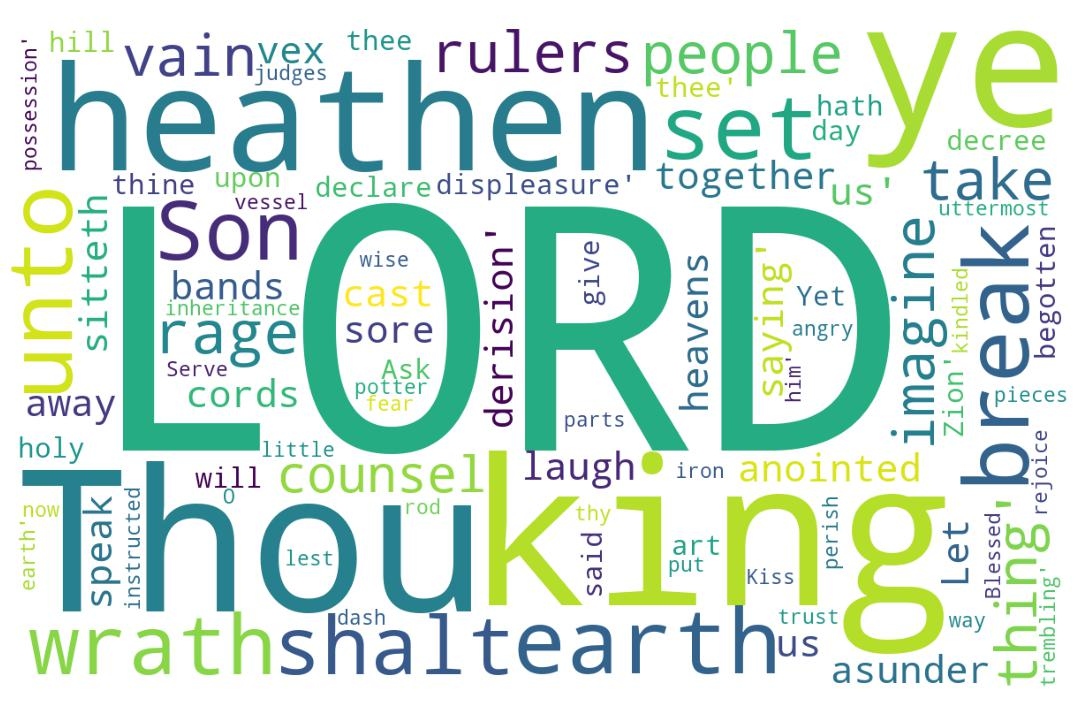
\includegraphics[width=\linewidth]{19OT-Psalms/Psalm2-WordCloud.jpg}
  \caption{Psalm 2 Word Cloud}
  \label{fig:Psalm 2 word Cloud}
\end{figure}


\marginpar{\scriptsize \centering \fcolorbox{bone}{lime}{\textbf{WHY THE HEATHEN RAGE (I)}}\\ (Psalm 2:1-12) 
\begin{compactenum}[I.][8]
    \item They have no \textbf{Savior}
    \item They have no \textbf{Seed}
    \item They have no \textbf{Seekers}
    \item They have no \textbf{Supplication}
    \item They have no \textbf{Security}
    \item They have no \textbf{Substance}
    \item They have no \textbf{Salvation}
\end{compactenum} }

\marginpar{\scriptsize \centering \fcolorbox{bone}{yellow}{\textbf{WHY THE HEATHEN RAGE (II)}}\\ (Psalm 2:1-12) 
\begin{compactenum}[I.][8]
    \item \textbf{Utter Rebellion} (Futility) \index[scripture]{Psalms!Psa 002:01-03} (Psa 2:1-3)
    \item \textbf{Undaunted Religion} (Ferocity) \index[scripture]{Psalms!Psa 002:04-06} (Psa 2:4-6)
    \item \textbf{Unrestrained Ridicule} \index[scripture]{Psalms!Psa 002:04} (Psa 2:4)
    \item \textbf{Ultimate Reign} (Finality) \index[scripture]{Psalms!Psa 002:07-09} (Psa 2:7-9)
    \item \textbf{Untimely Return} (Fire) \index[scripture]{Psalms!Psa 002:09} (Psa 2:9)
    \item \textbf{Unmitigated Ruin} (Finish) \index[scripture]{Psalms!Psa 002:09} (Psa 2:9)
    \item \textbf{Urgent Recommendation} (Fear) \index[scripture]{Psalms!Psa 002:10-12} (Psa 2:10-12)
    \item \textbf{Un-applied Repentance} (Forgiveness) \index[scripture]{Psalms!Psa 002:12} (Psa 2:12)
\end{compactenum} }

\marginpar{\scriptsize \centering \fcolorbox{bone}{black}{\textcolor{white}{\textbf{MAN, KNOWING HIS PLACE}}}\\ (Psalm 2:1-12) 
\begin{compactenum}[I.][8]
    \item The \textbf{Rage}  \index[scripture]{Psalms!Psa 002:01} (Psa 2:1)
    \item The \textbf{Rebellion}  \index[scripture]{Psalms!Psa 002:02} (Psa 2:2)
    \item The \textbf{Restraint}  \index[scripture]{Psalms!Psa 002:03} (Psa 2:3)
    \item The \textbf{Ruin}  \index[scripture]{Psalms!Psa 002:09} (Psa 2:9)
    \item The \textbf{Repentance}  \index[scripture]{Psalms!Psa 002:11} (Psa 2:11)
    \item The \textbf{Rejoicing}  \index[scripture]{Psalms!Psa 002:01} (Psa 2:1)
    \item The \textbf{Reality}  \index[scripture]{Psalms!Psa 002:12} (Psa 2:12)
\end{compactenum} }

\footnote{\textcolor[cmyk]{0.99998,1,0,0}{\hyperlink{TOC}{Return to end of Table of Contents.}}}\footnote{\href{https://www.audioverse.org/english/audiobibles/books/ENGKJV/O/Ps/1}{\textcolor[cmyk]{0.99998,1,0,0}{Psalms Audio}}}\textcolor[cmyk]{0.99998,1,0,0}{Why\textcolor{jungle}{$_{131}$} do the heathen rage, and the people imagine a vain thing?}
[2] \textcolor[cmyk]{0.99998,1,0,0}{The\textcolor{jungle}{$_{143}$} kings of the earth set themselves, and the rulers take \fcolorbox{bone}{yellow}{counsel} together, against the LORD, and against his anointed, \emph{saying},}
[3] \textcolor[cmyk]{0.99998,1,0,0}{Let\textcolor{jungle}{$_{164}$} us break their bands asunder, and cast away their cords from us.}
[4] \textcolor[cmyk]{0.99998,1,0,0}{He\textcolor{jungle}{$_{177}$} that sitteth in the heavens shall \fcolorbox{bone}{yellow}{laugh}: the Lord shall have them in \fcolorbox{bone}{yellow}{derision}.}
[5] \textcolor[cmyk]{0.99998,1,0,0}{Then\textcolor{jungle}{$_{192}$} shall he speak unto them in his \fcolorbox{bone}{yellow}{wrath}, and vex them in his sore displeasure.}
[6] \textcolor[cmyk]{0.99998,1,0,0}{Yet\textcolor{jungle}{$_{208}$} have I set my king upon my holy hill of Zion.}
[7] \textcolor[cmyk]{0.99998,1,0,0}{I\textcolor{jungle}{$_{220}$} will declare the decree: the LORD hath said unto me, Thou \emph{art} my Son; this day have I begotten thee.}
[8] \textcolor[cmyk]{0.99998,1,0,0}{Ask\textcolor{jungle}{$_{241}$} of me, and I shall give \emph{thee} the heathen \emph{for} \fcolorbox{bone}{yellow}{thine inheritance}, and the uttermost parts of the earth \emph{for} thy possession.}
[9] \textcolor[cmyk]{0.99998,1,0,0}{Thou\textcolor{jungle}{$_{264}$} shalt \fcolorbox{bone}{yellow}{break them} with a rod of iron; thou shalt \fcolorbox{bone}{yellow}{dash them} in pieces like a potter's vessel.}
[10] \textcolor[cmyk]{0.99998,1,0,0}{\fcolorbox{bone}{yellow}{Be}\textcolor{jungle}{$_{283}$} \fcolorbox{bone}{yellow}{wise} now therefore, O ye kings: be instructed, ye judges of the earth.}
[11] \textcolor[cmyk]{0.99998,1,0,0}{Serve\textcolor{jungle}{$_{297}$} the LORD with fear, and rejoice with trembling.}
[12] \textcolor[cmyk]{0.99998,1,0,0}{\fcolorbox{bone}{yellow}{Kiss\textcolor{jungle}{$_{306}$} the Son}, lest he be angry, and ye perish \emph{from} the way, when his wrath is kindled but a little. Blessed \emph{are} all they that put their trust in him\textcolor{jungle}{$_{336}$}.}


\section{Psalm 2 Comments}



\subsection{Psalm 2:1, 2}
Modern translations corrupt this verse.\footnote{\textbf{Isaiah 40:17} - All nations before him are as nothing; and they are counted to him less than nothing, and vanity.} But these heathen are everywhere.  The rage. They rule.  They rise up. They mostly reject. They ruin things.  Theses heathen are the ones to whome the gospel is to be preached in Galatians 1:16, 2:9, and 3:8.\footnote{\textbf{Galatians 1:16} - To reveal his Son in me, that I might preach him among the heathen; immediately I conferred not with flesh and blood:}\footnote{\textbf{Galatians 2:9} - And when James, Cephas, and John, who seemed to be pillars, perceived the grace that was given unto me, they gave to me and Barnabas the right hands of fellowship; that we should go unto the heathen, and they unto the circumcision.}\footnote{\textbf{Galatians 3:8} - And the scripture, foreseeing that God would justify the heathen through faith, preached before the gospel unto Abraham, saying, In thee shall all nations be blessed.}\\
\\
\noindent Verses 1 and 2 are used in Acts 4:27 to describe the collection of Pilate, Herod, the Gentiles, Christ-rejecting Israelites, organized religion, and organized politics, to rise up and destroy God's work on Earth.  But this rebellion was only partially fulfilled.\cite{Ruckman1992PsalmsV1} The future focus of united mankind (typified in Genesis 11) will be this rebellion.
%%%%%%%%%%%%%%%%%%%%%%%%%%%%%%%%%%%%%%%%%%%%%%%%%

%%%%%%%%%%%%%%%%%%%%%%%%%%%%%%%%%%%%%%%%%%%%%%%%

\begin{center}

\begin{table}[ht]
\centering
\begin{tabular}{|p{.5in}|p{3.5in}|}
\hline

\textcolor[rgb]{0.00,0.00,1.00}{AV} & \textcolor[rgb]{0.00,0.00,1.00}{Why do the heathen rage, and the people imagine a vain thing?} \\ 
\hline \hline

ASV &  Why do the nations rage, And the peoples meditate a vain thing? \\ \hline
%
CEB &  Why do the nations rant?   Why do the peoples rave uselessly?\\ \hline
%
ESV & Why do the nations rage and the peoples plot in vain? \\ \hline
%
NASV &  Why are the nations restless And the peoples plotting in vain? \\ \hline
%
MEV & Why do the nations rage,  and the peoples plot in vain?\\ \hline
%
NIV &  Why do the nations conspire  and the peoples plot in vain? \\ \hline
%
NKJV &  Why do the nations rage, And the people plot a vain thing? \\ \hline
%
RSV &  Why do the nations conspire, and the peoples plot in vain?\\ \hline \hline

\multicolumn{2}{|p{4.2in}|}{{\textcolor{jungle}{Modern translations soften and dilute the verse by changing the word `heathen'' to ``nations.'' It is almnost as if to say that only some of the ``nations'' are ``heathen.'' These nations are  identified in Isaiah 40:17.}}} \\ \hline

\end{tabular}
\caption[Corruption Alert: Psalm 2:1]{Corruption Alert: Psalm 2:1} \label{table:CorruptionPsalm-2-1}
\end{table}

\end{center}

%%%%%%%%%%%%%%%%%%%%%%%%%%%%%%%%%%%%%%%%%%%%%%%%





\subsection{Psalm 2:3}
There are some sort of ``bands'' and ``cords'' that are currently preventing the conclusion of this rage. Something like this is described in Isaiah 30:28 and Matthew 13:30. Something like this is described in 2 Thessalonians 2:6.\footnote{\textbf{Isaiah 30:28} - And his breath, as an overflowing stream, shall reach to the midst of the neck, to sift the nations with the sieve of vanity: and there shall be a bridle in the jaws of the people, causing them to err.}\footnote{\textbf{Matthew 13:30} - The field is the world; the good seed are the children of the kingdom; but the tares are the children of the wicked one;}\footnote{\textbf{2 Thessalonians 2:6} - And now ye know what withholdeth that he might be revealed in his time.} \cite{Ruckman1992PsalmsV1}

%\index[NWIV]{12!Psalms!Psa 2:1}\index[AWIP]{Why!Psalms!Psa 2:1}\index[AWIP]{do!Psalms!Psa 2:1}\index[AWIP]{the!Psalms!Psa 2:1}\index[AWIP]{the!Psalms!Psa 2:1 (2)}\index[AWIP]{heathen!Psalms!Psa 2:1}\index[AWIP]{rage!Psalms!Psa 2:1}\index[AWIP]{and!Psalms!Psa 2:1}\index[AWIP]{people!Psalms!Psa 2:1}\index[AWIP]{imagine!Psalms!Psa 2:1}\index[AWIP]{a!Psalms!Psa 2:1}\index[AWIP]{vain!Psalms!Psa 2:1}\index[AWIP]{thing?!Psalms!Psa 2:1}

\index[NWIV]{21!Psalms!Psa 2:2}\index[AWIP]{The!Psalms!Psa 2:2}\index[AWIP]{kings!Psalms!Psa 2:2}\index[AWIP]{of!Psalms!Psa 2:2}\index[AWIP]{the!Psalms!Psa 2:2}\index[AWIP]{the!Psalms!Psa 2:2 (2)}\index[AWIP]{the!Psalms!Psa 2:2 (3)}\index[AWIP]{earth!Psalms!Psa 2:2}\index[AWIP]{set!Psalms!Psa 2:2}\index[AWIP]{themselves!Psalms!Psa 2:2}\index[AWIP]{and!Psalms!Psa 2:2}\index[AWIP]{and!Psalms!Psa 2:2 (2)}\index[AWIP]{rulers!Psalms!Psa 2:2}\index[AWIP]{take!Psalms!Psa 2:2}\index[AWIP]{counsel!Psalms!Psa 2:2}\index[AWIP]{together!Psalms!Psa 2:2}\index[AWIP]{against!Psalms!Psa 2:2}\index[AWIP]{against!Psalms!Psa 2:2 (2)}\index[AWIP]{LORD!Psalms!Psa 2:2}\index[AWIP]{his!Psalms!Psa 2:2}\index[AWIP]{anointed!Psalms!Psa 2:2}\index[AWIP]{\emph{saying}!Psalms!Psa 2:2}\index[AWIP]{\emph{saying}!Psalms!Psa 2:2}

\index[NWIV]{13!Psalms!Psa 2:3}\index[AWIP]{Let!Psalms!Psa 2:3}\index[AWIP]{us!Psalms!Psa 2:3}\index[AWIP]{us!Psalms!Psa 2:3 (2)}\index[AWIP]{break!Psalms!Psa 2:3}\index[AWIP]{their!Psalms!Psa 2:3}\index[AWIP]{their!Psalms!Psa 2:3 (2)}\index[AWIP]{bands!Psalms!Psa 2:3}\index[AWIP]{asunder!Psalms!Psa 2:3}\index[AWIP]{and!Psalms!Psa 2:3}\index[AWIP]{cast!Psalms!Psa 2:3}\index[AWIP]{away!Psalms!Psa 2:3}\index[AWIP]{cords!Psalms!Psa 2:3}\index[AWIP]{from!Psalms!Psa 2:3}

\index[NWIV]{15!Psalms!Psa 2:4}\index[AWIP]{He!Psalms!Psa 2:4}\index[AWIP]{that!Psalms!Psa 2:4}\index[AWIP]{sitteth!Psalms!Psa 2:4}\index[AWIP]{in!Psalms!Psa 2:4}\index[AWIP]{in!Psalms!Psa 2:4 (2)}\index[AWIP]{the!Psalms!Psa 2:4}\index[AWIP]{the!Psalms!Psa 2:4 (2)}\index[AWIP]{heavens!Psalms!Psa 2:4}\index[AWIP]{shall!Psalms!Psa 2:4}\index[AWIP]{shall!Psalms!Psa 2:4 (2)}\index[AWIP]{laugh!Psalms!Psa 2:4}\index[AWIP]{Lord!Psalms!Psa 2:4}\index[AWIP]{have!Psalms!Psa 2:4}\index[AWIP]{them!Psalms!Psa 2:4}\index[AWIP]{derision!Psalms!Psa 2:4}

\index[NWIV]{16!Psalms!Psa 2:5}\index[AWIP]{Then!Psalms!Psa 2:5}\index[AWIP]{shall!Psalms!Psa 2:5}\index[AWIP]{he!Psalms!Psa 2:5}\index[AWIP]{speak!Psalms!Psa 2:5}\index[AWIP]{unto!Psalms!Psa 2:5}\index[AWIP]{them!Psalms!Psa 2:5}\index[AWIP]{them!Psalms!Psa 2:5 (2)}\index[AWIP]{in!Psalms!Psa 2:5}\index[AWIP]{in!Psalms!Psa 2:5 (2)}\index[AWIP]{his!Psalms!Psa 2:5}\index[AWIP]{his!Psalms!Psa 2:5 (2)}\index[AWIP]{wrath!Psalms!Psa 2:5}\index[AWIP]{and!Psalms!Psa 2:5}\index[AWIP]{vex!Psalms!Psa 2:5}\index[AWIP]{sore!Psalms!Psa 2:5}\index[AWIP]{displeasure!Psalms!Psa 2:5}

\index[NWIV]{12!Psalms!Psa 2:6}\index[AWIP]{Yet!Psalms!Psa 2:6}\index[AWIP]{have!Psalms!Psa 2:6}\index[AWIP]{I!Psalms!Psa 2:6}\index[AWIP]{set!Psalms!Psa 2:6}\index[AWIP]{my!Psalms!Psa 2:6}\index[AWIP]{my!Psalms!Psa 2:6 (2)}\index[AWIP]{king!Psalms!Psa 2:6}\index[AWIP]{upon!Psalms!Psa 2:6}\index[AWIP]{holy!Psalms!Psa 2:6}\index[AWIP]{hill!Psalms!Psa 2:6}\index[AWIP]{of!Psalms!Psa 2:6}\index[AWIP]{Zion!Psalms!Psa 2:6}

\index[NWIV]{21!Psalms!Psa 2:7}\index[AWIP]{I!Psalms!Psa 2:7}\index[AWIP]{I!Psalms!Psa 2:7 (2)}\index[AWIP]{will!Psalms!Psa 2:7}\index[AWIP]{declare!Psalms!Psa 2:7}\index[AWIP]{the!Psalms!Psa 2:7}\index[AWIP]{the!Psalms!Psa 2:7 (2)}\index[AWIP]{decree!Psalms!Psa 2:7}\index[AWIP]{LORD!Psalms!Psa 2:7}\index[AWIP]{hath!Psalms!Psa 2:7}\index[AWIP]{said!Psalms!Psa 2:7}\index[AWIP]{unto!Psalms!Psa 2:7}\index[AWIP]{me!Psalms!Psa 2:7}\index[AWIP]{Thou!Psalms!Psa 2:7}\index[AWIP]{\emph{art}!Psalms!Psa 2:7}\index[AWIP]{my!Psalms!Psa 2:7}\index[AWIP]{Son!Psalms!Psa 2:7}\index[AWIP]{this!Psalms!Psa 2:7}\index[AWIP]{day!Psalms!Psa 2:7}\index[AWIP]{have!Psalms!Psa 2:7}\index[AWIP]{begotten!Psalms!Psa 2:7}\index[AWIP]{thee!Psalms!Psa 2:7}\index[AWIP]{\emph{art}!Psalms!Psa 2:7}

\index[NWIV]{23!Psalms!Psa 2:8}\index[AWIP]{Ask!Psalms!Psa 2:8}\index[AWIP]{of!Psalms!Psa 2:8}\index[AWIP]{of!Psalms!Psa 2:8 (2)}\index[AWIP]{me!Psalms!Psa 2:8}\index[AWIP]{and!Psalms!Psa 2:8}\index[AWIP]{and!Psalms!Psa 2:8 (2)}\index[AWIP]{I!Psalms!Psa 2:8}\index[AWIP]{shall!Psalms!Psa 2:8}\index[AWIP]{give!Psalms!Psa 2:8}\index[AWIP]{\emph{thee}!Psalms!Psa 2:8}\index[AWIP]{the!Psalms!Psa 2:8}\index[AWIP]{the!Psalms!Psa 2:8 (2)}\index[AWIP]{the!Psalms!Psa 2:8 (3)}\index[AWIP]{heathen!Psalms!Psa 2:8}\index[AWIP]{\emph{for}!Psalms!Psa 2:8}\index[AWIP]{\emph{for}!Psalms!Psa 2:8 (2)}\index[AWIP]{thine!Psalms!Psa 2:8}\index[AWIP]{inheritance!Psalms!Psa 2:8}\index[AWIP]{uttermost!Psalms!Psa 2:8}\index[AWIP]{parts!Psalms!Psa 2:8}\index[AWIP]{earth!Psalms!Psa 2:8}\index[AWIP]{thy!Psalms!Psa 2:8}\index[AWIP]{possession!Psalms!Psa 2:8}\index[AWIP]{\emph{thee}!Psalms!Psa 2:8}\index[AWIP]{\emph{for}!Psalms!Psa 2:8}\index[AWIP]{\emph{for}!Psalms!Psa 2:8 (2)}

\index[NWIV]{19!Psalms!Psa 2:9}\index[AWIP]{Thou!Psalms!Psa 2:9}\index[AWIP]{shalt!Psalms!Psa 2:9}\index[AWIP]{shalt!Psalms!Psa 2:9 (2)}\index[AWIP]{break!Psalms!Psa 2:9}\index[AWIP]{them!Psalms!Psa 2:9}\index[AWIP]{them!Psalms!Psa 2:9 (2)}\index[AWIP]{with!Psalms!Psa 2:9}\index[AWIP]{a!Psalms!Psa 2:9}\index[AWIP]{a!Psalms!Psa 2:9 (2)}\index[AWIP]{rod!Psalms!Psa 2:9}\index[AWIP]{of!Psalms!Psa 2:9}\index[AWIP]{iron!Psalms!Psa 2:9}\index[AWIP]{thou!Psalms!Psa 2:9}\index[AWIP]{dash!Psalms!Psa 2:9}\index[AWIP]{in!Psalms!Psa 2:9}\index[AWIP]{pieces!Psalms!Psa 2:9}\index[AWIP]{like!Psalms!Psa 2:9}\index[AWIP]{potter's!Psalms!Psa 2:9}\index[AWIP]{vessel!Psalms!Psa 2:9}

\index[NWIV]{14!Psalms!Psa 2:10}\index[AWIP]{Be!Psalms!Psa 2:10}\index[AWIP]{wise!Psalms!Psa 2:10}\index[AWIP]{now!Psalms!Psa 2:10}\index[AWIP]{therefore!Psalms!Psa 2:10}\index[AWIP]{O!Psalms!Psa 2:10}\index[AWIP]{ye!Psalms!Psa 2:10}\index[AWIP]{ye!Psalms!Psa 2:10 (2)}\index[AWIP]{kings!Psalms!Psa 2:10}\index[AWIP]{be!Psalms!Psa 2:10}\index[AWIP]{instructed!Psalms!Psa 2:10}\index[AWIP]{judges!Psalms!Psa 2:10}\index[AWIP]{of!Psalms!Psa 2:10}\index[AWIP]{the!Psalms!Psa 2:10}\index[AWIP]{earth!Psalms!Psa 2:10}

\index[NWIV]{9!Psalms!Psa 2:11}\index[AWIP]{Serve!Psalms!Psa 2:11}\index[AWIP]{the!Psalms!Psa 2:11}\index[AWIP]{LORD!Psalms!Psa 2:11}\index[AWIP]{with!Psalms!Psa 2:11}\index[AWIP]{with!Psalms!Psa 2:11 (2)}\index[AWIP]{fear!Psalms!Psa 2:11}\index[AWIP]{and!Psalms!Psa 2:11}\index[AWIP]{rejoice!Psalms!Psa 2:11}\index[AWIP]{trembling!Psalms!Psa 2:11}

\index[NWIV]{31!Psalms!Psa 2:12}\index[AWIP]{Kiss!Psalms!Psa 2:12}\index[AWIP]{the!Psalms!Psa 2:12}\index[AWIP]{the!Psalms!Psa 2:12 (2)}\index[AWIP]{Son!Psalms!Psa 2:12}\index[AWIP]{lest!Psalms!Psa 2:12}\index[AWIP]{he!Psalms!Psa 2:12}\index[AWIP]{be!Psalms!Psa 2:12}\index[AWIP]{angry!Psalms!Psa 2:12}\index[AWIP]{and!Psalms!Psa 2:12}\index[AWIP]{ye!Psalms!Psa 2:12}\index[AWIP]{perish!Psalms!Psa 2:12}\index[AWIP]{\emph{from}!Psalms!Psa 2:12}\index[AWIP]{way!Psalms!Psa 2:12}\index[AWIP]{when!Psalms!Psa 2:12}\index[AWIP]{his!Psalms!Psa 2:12}\index[AWIP]{wrath!Psalms!Psa 2:12}\index[AWIP]{is!Psalms!Psa 2:12}\index[AWIP]{kindled!Psalms!Psa 2:12}\index[AWIP]{but!Psalms!Psa 2:12}\index[AWIP]{a!Psalms!Psa 2:12}\index[AWIP]{little!Psalms!Psa 2:12}\index[AWIP]{Blessed!Psalms!Psa 2:12}\index[AWIP]{\emph{are}!Psalms!Psa 2:12}\index[AWIP]{all!Psalms!Psa 2:12}\index[AWIP]{they!Psalms!Psa 2:12}\index[AWIP]{that!Psalms!Psa 2:12}\index[AWIP]{put!Psalms!Psa 2:12}\index[AWIP]{their!Psalms!Psa 2:12}\index[AWIP]{trust!Psalms!Psa 2:12}\index[AWIP]{in!Psalms!Psa 2:12}\index[AWIP]{him!Psalms!Psa 2:12}\index[AWIP]{\emph{from}!Psalms!Psa 2:12}\index[AWIP]{\emph{are}!Psalms!Psa 2:12}


\section{Psalm 2 Outlines}

\subsection{My Outlines}

\subsubsection{Why Do the Heathen Rage}
\index[speaker]{Keith Anthony!Psalm 002 (Why Do the Heathen Rage I)}
\index[series]{Psalms (Keith Anthony)!Psalm 002 (Why Do the Heathen Rage I)}
\index[date]{2016/06/08!Psalm 002 (Why Do the Heathen Rage I) (Keith Anthony)}
\begin{compactenum}[I.][19]
    \item They have no \textbf{Savior}
    \item They have no \textbf{Seed}
    \item They have no \textbf{Seekers}
    \item They have no \textbf{Supplication}
    \item They have no \textbf{Security}
    \item They have no \textbf{Substance}
    \item They have no \textbf{Salvation}
\end{compactenum}

\subsubsection{Why Do the Heathen Rage (II)}

\index[speaker]{Keith Anthony!Psalm 002 (Why Do the Heathen Rage II)}
\index[series]{Psalms (Keith Anthony)!Psalm 002 (Why Do the Heathen Rage II)}
\index[date]{2016/06/08!Psalm 002 (Why Do the Heathen Rage II) (Keith Anthony)}
\begin{compactenum}[I.][19]
    \item \textbf{Utter Rebellion} (Futility) \index[scripture]{Psalms!Psa 002:01-03} (Psa 2:1-3)
    \item \textbf{Undaunted Religion} (Ferocity) \index[scripture]{Psalms!Psa 002:04-06} (Psa 2:4-6)
    \item \textbf{Unrestrained Ridicule} \index[scripture]{Psalms!Psa 002:04} (Psa 2:4)
    \item \textbf{Ultimate Reign} (Finality) \index[scripture]{Psalms!Psa 002:07-09} (Psa 2:7-9)
    \item \textbf{Untimely Return} (Fire) \index[scripture]{Psalms!Psa 002:09} (Psa 2:9)
    \item \textbf{Unmitigated Ruin} (Finish) \index[scripture]{Psalms!Psa 002:09} (Psa 2:9)
    \item \textbf{Urgent Recommendation} (Fear) \index[scripture]{Psalms!Psa 002:10-12} (Psa 2:10-12)
    \item \textbf{Un-applied Repentance} (Forgiveness) \index[scripture]{Psalms!Psa 002:12} (Psa 2:12)
\end{compactenum}

\subsubsection{Man, Knowing His Place}

\index[speaker]{Keith Anthony!Psalm 002 (Man, Knowing His Place)}
\index[series]{Psalms (Keith Anthony)!Psalm 002 (Man, Knowing His Place)}
\index[date]{2021/01/02!Psalm 002 (Man, Knowing His Place) (Keith Anthony)}
\begin{compactenum}[I.][8]
    \item The \textbf{Rage}  \index[scripture]{Psalms!Psa 002:01} (Psa 2:1)
    \item The \textbf{Rebellion}  \index[scripture]{Psalms!Psa 002:02} (Psa 2:2)
    \item The \textbf{Restraint}  \index[scripture]{Psalms!Psa 002:03} (Psa 2:3)
    \item The \textbf{Ruin}  \index[scripture]{Psalms!Psa 002:09} (Psa 2:9)
    \item The \textbf{Repentance}  \index[scripture]{Psalms!Psa 002:11} (Psa 2:11)
    \item The \textbf{Rejoicing}  \index[scripture]{Psalms!Psa 002:01} (Psa 2:1)
    \item The \textbf{Reality}  \index[scripture]{Psalms!Psa 002:12} (Psa 2:12)
\end{compactenum} 


\subsection{Outlines from Others}

\subsubsection{The Program}
\textbf{Source: } Daniel The Prophet\cite{dehaan1995daniel}
\index[speaker]{M. R. Dehaan!Psalm 002 (The Program)}
\index[series]{Psalms (M. R. Dehaan)!Psalm 002 (The Program)}
\index[date]{M. R. Dehaan!Psalm 002 (The Program) (M. R. Dehaan)}
\begin{compactenum}[I.][19]
    \item \textbf{The Silent Lord on the Throne} \index[scripture]{Psalms!Psa 002:01-03} Psalm 2:1-3
    \item \textbf{The Laughing Lord of the Nations} \index[scripture]{Psalms!Psa 002:04} Psalm 2:4
    \item \textbf{The Speaking Lord from Heaven} \index[scripture]{Psalms!Psa 002:05} Psalm 2:5
    \item \textbf{The Judging Lord} \index[scripture]{Psalms!Psa 002:06--09} Psalm 2:6-9
    \item \textbf{The Reigning Lord of the Earth Heaven} \index[scripture]{Psalms!Psa 002:06--09} Psalm 2:6-9
    \item \textbf{The Warning Lord of Patience} \index[scripture]{Psalms!Psa 002:10--11} Psalm 2:10-11
    \item \textbf{The Saving Lord of Love} \index[scripture]{Psalms!Psa 002:12} Psalm 2:12
 \end{compactenum}




%\section{Psalm 2 Statistics}

%%%%%%%%%%%%%%%%%%%%%%%%%%%
%%%%%Word Statistics
%%%%%%%%%%%%%%%%%%%%%%%%%%%


\normalsize



\subsection{Chapter Word Statistics}


%%%%%%%%%%
%%%%%%%%%%
 
\begin{center}
\begin{longtable}{l|c|c|c|c}
\caption[Stats for Psalm 2]{Stats for Psalm 2} \label{table:Stats for Psalm 2} \\ 
\hline \multicolumn{1}{|c|}{\textbf{Verse(s)}} & \multicolumn{1}{|c|}{\textbf{Count}} & \multicolumn{1}{|c|}{\textbf{Unique}} & \multicolumn{1}{|c|}{\textbf{Italics}} & \multicolumn{1}{|c|}{\textbf{Uniq Italic}}  \\ \hline 
\endfirsthead
 
\multicolumn{5}{c}
{{\bfseries \tablename\ \thetable{} -- continued from previous page}} \\  
\hline \multicolumn{1}{|c|}{\textbf{Verse(s)}} & \multicolumn{1}{|c|}{\textbf{Count}} & \multicolumn{1}{|c|}{\textbf{Unique}} & \multicolumn{1}{|c|}{\textbf{Italics}} & \multicolumn{1}{|c|}{\textbf{Uniq Italic}}  \\ \hline 
\endhead
 
\hline \multicolumn{5}{|r|}{{Continued if needed}} \\ \hline
\endfoot 
1 & 12 & 11 & 0 & 0\\ \hline
2 & 21 & 17 & 1 & 1\\ \hline
3 & 13 & 11 & 0 & 0\\ \hline
4 & 15 & 12 & 0 & 0\\ \hline
5 & 16 & 13 & 0 & 0\\ \hline
6 & 12 & 11 & 0 & 0\\ \hline
7 & 21 & 19 & 1 & 1\\ \hline
8 & 23 & 18 & 3 & 2\\ \hline
9 & 19 & 16 & 0 & 0\\ \hline
10 & 14 & 13 & 0 & 0\\ \hline
11 & 9 & 8 & 0 & 0\\ \hline
12 & 31 & 30 & 2 & 2\\ \hline
\hline \hline
Total & 206 & 127 & 7 & 6



\end{longtable}
\end{center}

%%%%%%%%%%
%%%%%%%%%%
 
\subsection{Words by Frequency}

\begin{center}
\begin{longtable}{l|r}
\caption[Word Frequencies in Psalm 2]{Word Frequencies in Psalm 2} \label{table:WordsIn-Psalm-2} \\ 
\hline \multicolumn{1}{|c|}{\textbf{Word}} & \multicolumn{1}{c|}{\textbf{Frequency}} \\ \hline 
\endfirsthead
 
\multicolumn{2}{c}
{{\bfseries \tablename\ \thetable{} -- continued from previous page}} \\ 
\hline \multicolumn{1}{|c|}{\textbf{Word}} & \multicolumn{1}{c|}{\textbf{Frequency}} \\ \hline 
\endhead
 
\hline \multicolumn{2}{|r|}{{Continued if needed}} \\ \hline
\endfoot
 
\hline \hline
\endlastfoot
the & 16 \\ \hline
and & 9 \\ \hline
of & 6 \\ \hline
in & 6 \\ \hline
them & 5 \\ \hline
a & 4 \\ \hline
his & 4 \\ \hline
shall & 4 \\ \hline
I & 4 \\ \hline
earth & 3 \\ \hline
LORD & 3 \\ \hline
their & 3 \\ \hline
have & 3 \\ \hline
my & 3 \\ \hline
with & 3 \\ \hline
ye & 3 \\ \hline
heathen & 2 \\ \hline
kings & 2 \\ \hline
set & 2 \\ \hline
against & 2 \\ \hline
us & 2 \\ \hline
break & 2 \\ \hline
that & 2 \\ \hline
he & 2 \\ \hline
unto & 2 \\ \hline
wrath & 2 \\ \hline
me & 2 \\ \hline
Thou & 2 \\ \hline
Son & 2 \\ \hline
\emph{for} & 2 \\ \hline
shalt & 2 \\ \hline
be & 2 \\ \hline
Why & 1 \\ \hline
do & 1 \\ \hline
rage & 1 \\ \hline
people & 1 \\ \hline
imagine & 1 \\ \hline
vain & 1 \\ \hline
thing & 1 \\ \hline
The & 1 \\ \hline
themselves & 1 \\ \hline
rulers & 1 \\ \hline
take & 1 \\ \hline
counsel & 1 \\ \hline
together & 1 \\ \hline
anointed & 1 \\ \hline
\emph{saying} & 1 \\ \hline
Let & 1 \\ \hline
bands & 1 \\ \hline
asunder & 1 \\ \hline
cast & 1 \\ \hline
away & 1 \\ \hline
cords & 1 \\ \hline
from & 1 \\ \hline
He & 1 \\ \hline
sitteth & 1 \\ \hline
heavens & 1 \\ \hline
laugh & 1 \\ \hline
Lord & 1 \\ \hline
derision & 1 \\ \hline
Then & 1 \\ \hline
speak & 1 \\ \hline
vex & 1 \\ \hline
sore & 1 \\ \hline
displeasure & 1 \\ \hline
Yet & 1 \\ \hline
king & 1 \\ \hline
upon & 1 \\ \hline
holy & 1 \\ \hline
hill & 1 \\ \hline
Zion & 1 \\ \hline
will & 1 \\ \hline
declare & 1 \\ \hline
decree & 1 \\ \hline
hath & 1 \\ \hline
said & 1 \\ \hline
\emph{art} & 1 \\ \hline
this & 1 \\ \hline
day & 1 \\ \hline
begotten & 1 \\ \hline
thee & 1 \\ \hline
Ask & 1 \\ \hline
give & 1 \\ \hline
\emph{thee} & 1 \\ \hline
thine & 1 \\ \hline
inheritance & 1 \\ \hline
uttermost & 1 \\ \hline
parts & 1 \\ \hline
thy & 1 \\ \hline
possession & 1 \\ \hline
rod & 1 \\ \hline
iron & 1 \\ \hline
thou & 1 \\ \hline
dash & 1 \\ \hline
pieces & 1 \\ \hline
like & 1 \\ \hline
potter's & 1 \\ \hline
vessel & 1 \\ \hline
Be & 1 \\ \hline
wise & 1 \\ \hline
now & 1 \\ \hline
therefore & 1 \\ \hline
O & 1 \\ \hline
instructed & 1 \\ \hline
judges & 1 \\ \hline
Serve & 1 \\ \hline
fear & 1 \\ \hline
rejoice & 1 \\ \hline
trembling & 1 \\ \hline
Kiss & 1 \\ \hline
lest & 1 \\ \hline
angry & 1 \\ \hline
perish & 1 \\ \hline
\emph{from} & 1 \\ \hline
way & 1 \\ \hline
when & 1 \\ \hline
is & 1 \\ \hline
kindled & 1 \\ \hline
but & 1 \\ \hline
little & 1 \\ \hline
Blessed & 1 \\ \hline
\emph{are} & 1 \\ \hline
all & 1 \\ \hline
they & 1 \\ \hline
put & 1 \\ \hline
trust & 1 \\ \hline
him & 1 \\ \hline
\end{longtable}
\end{center}



\normalsize



\subsection{Words Alphabetically}

\begin{center}
\begin{longtable}{l|r}
\caption[Word Alphabetically in Psalm 2]{Word Alphabetically in Psalm 2} \label{table:WordsIn-Psalm-2} \\ 
\hline \multicolumn{1}{|c|}{\textbf{Word}} & \multicolumn{1}{c|}{\textbf{Frequency}} \\ \hline 
\endfirsthead
 
\multicolumn{2}{c}
{{\bfseries \tablename\ \thetable{} -- continued from previous page}} \\ 
\hline \multicolumn{1}{|c|}{\textbf{Word}} & \multicolumn{1}{c|}{\textbf{Frequency}} \\ \hline 
\endhead
 
\hline \multicolumn{2}{|r|}{{Continued if needed}} \\ \hline
\endfoot
 
\hline \hline
\endlastfoot
Ask & 1 \\ \hline
Be & 1 \\ \hline
Blessed & 1 \\ \hline
He & 1 \\ \hline
I & 4 \\ \hline
Kiss & 1 \\ \hline
LORD & 3 \\ \hline
Let & 1 \\ \hline
Lord & 1 \\ \hline
O & 1 \\ \hline
Serve & 1 \\ \hline
Son & 2 \\ \hline
The & 1 \\ \hline
Then & 1 \\ \hline
Thou & 2 \\ \hline
Why & 1 \\ \hline
Yet & 1 \\ \hline
Zion & 1 \\ \hline
\emph{are} & 1 \\ \hline
\emph{art} & 1 \\ \hline
\emph{for} & 2 \\ \hline
\emph{from} & 1 \\ \hline
\emph{saying} & 1 \\ \hline
\emph{thee} & 1 \\ \hline
a & 4 \\ \hline
against & 2 \\ \hline
all & 1 \\ \hline
and & 9 \\ \hline
angry & 1 \\ \hline
anointed & 1 \\ \hline
asunder & 1 \\ \hline
away & 1 \\ \hline
bands & 1 \\ \hline
be & 2 \\ \hline
begotten & 1 \\ \hline
break & 2 \\ \hline
but & 1 \\ \hline
cast & 1 \\ \hline
cords & 1 \\ \hline
counsel & 1 \\ \hline
dash & 1 \\ \hline
day & 1 \\ \hline
declare & 1 \\ \hline
decree & 1 \\ \hline
derision & 1 \\ \hline
displeasure & 1 \\ \hline
do & 1 \\ \hline
earth & 3 \\ \hline
fear & 1 \\ \hline
from & 1 \\ \hline
give & 1 \\ \hline
hath & 1 \\ \hline
have & 3 \\ \hline
he & 2 \\ \hline
heathen & 2 \\ \hline
heavens & 1 \\ \hline
hill & 1 \\ \hline
him & 1 \\ \hline
his & 4 \\ \hline
holy & 1 \\ \hline
imagine & 1 \\ \hline
in & 6 \\ \hline
inheritance & 1 \\ \hline
instructed & 1 \\ \hline
iron & 1 \\ \hline
is & 1 \\ \hline
judges & 1 \\ \hline
kindled & 1 \\ \hline
king & 1 \\ \hline
kings & 2 \\ \hline
laugh & 1 \\ \hline
lest & 1 \\ \hline
like & 1 \\ \hline
little & 1 \\ \hline
me & 2 \\ \hline
my & 3 \\ \hline
now & 1 \\ \hline
of & 6 \\ \hline
parts & 1 \\ \hline
people & 1 \\ \hline
perish & 1 \\ \hline
pieces & 1 \\ \hline
possession & 1 \\ \hline
potter's & 1 \\ \hline
put & 1 \\ \hline
rage & 1 \\ \hline
rejoice & 1 \\ \hline
rod & 1 \\ \hline
rulers & 1 \\ \hline
said & 1 \\ \hline
set & 2 \\ \hline
shall & 4 \\ \hline
shalt & 2 \\ \hline
sitteth & 1 \\ \hline
sore & 1 \\ \hline
speak & 1 \\ \hline
take & 1 \\ \hline
that & 2 \\ \hline
the & 16 \\ \hline
thee & 1 \\ \hline
their & 3 \\ \hline
them & 5 \\ \hline
themselves & 1 \\ \hline
therefore & 1 \\ \hline
they & 1 \\ \hline
thine & 1 \\ \hline
thing & 1 \\ \hline
this & 1 \\ \hline
thou & 1 \\ \hline
thy & 1 \\ \hline
together & 1 \\ \hline
trembling & 1 \\ \hline
trust & 1 \\ \hline
unto & 2 \\ \hline
upon & 1 \\ \hline
us & 2 \\ \hline
uttermost & 1 \\ \hline
vain & 1 \\ \hline
vessel & 1 \\ \hline
vex & 1 \\ \hline
way & 1 \\ \hline
when & 1 \\ \hline
will & 1 \\ \hline
wise & 1 \\ \hline
with & 3 \\ \hline
wrath & 2 \\ \hline
ye & 3 \\ \hline
\end{longtable}
\end{center}



\normalsize



\subsection{Word Lengths in Chapter}
\normalsize
\begin{longtable}{l|p{3.75in}}
\caption[Words by Length in Psalm 2]{Words by Length in Psalm 2} \label{table:WordsIn-Psalm-2} \\ 
\hline \multicolumn{1}{|c|}{\textbf{Length}} & \multicolumn{1}{c|}{\textbf{Words}} \\ \hline 
\endfirsthead
 
\multicolumn{2}{c}
{{\bfseries \tablename\ \thetable{} -- continued from previous page}} \\ 
\hline \multicolumn{1}{|c|}{\textbf{Length}} & \multicolumn{1}{c|}{\textbf{Words}} \\ \hline 
\endhead
 
\hline \multicolumn{2}{|r|}{{Continued if needed}} \\ \hline
\endfoot
 
\hline \hline
\endlastfoot
1 & a, I, O \\ \hline
2 & do, of, us, He, in, he, my, me, Be, ye, be, is \\ \hline
3 & Why, the, and, The, set, his, Let, vex, Yet, \emph{art}, Son, day, Ask, \emph{for}, thy, rod, now, way, but, \emph{are}, all, put, him \\ \hline
4 & rage, vain, take, LORD, cast, away, from, that, Lord, have, them, Then, unto, sore, king, upon, holy, hill, Zion, will, hath, said, Thou, this, thee, give, \emph{thee}, with, iron, thou, dash, like, wise, fear, Kiss, lest, \emph{from}, when, they \\ \hline
5 & thing, kings, earth, break, their, bands, cords, shall, laugh, speak, wrath, thine, parts, shalt, Serve, angry, trust \\ \hline
6 & people, rulers, \emph{saying}, decree, pieces, vessel, judges, perish, little \\ \hline
7 & heathen, imagine, counsel, against, asunder, sitteth, heavens, declare, rejoice, kindled, Blessed \\ \hline
8 & together, anointed, derision, begotten, potter's \\ \hline
9 & uttermost, therefore, trembling \\ \hline
10 & themselves, possession, instructed \\ \hline
11 & displeasure, inheritance \\ \hline
\end{longtable}






%%%%%%%%%%
%%%%%%%%%%
 



%%%%%%%%%%
%%%%%%%%%%
\subsection{Verses with 13 Words in Chapter}
\normalsize
\begin{longtable}{l|p{3.75in}}
\caption[Verses with 13 Words  in Psalm 2]{Verses with 13 Words  in Psalm 2} \label{table:Verses with 13 Words in-Psalm-2} \\ 
\hline \multicolumn{1}{|c|}{\textbf{Reference}} & \multicolumn{1}{c|}{\textbf{Verse}} \\ \hline 
\endfirsthead
 
\multicolumn{2}{c}
{{\bfseries \tablename\ \thetable{} -- continued from previous page}} \\ 
\hline \multicolumn{1}{|c|}{\textbf{Reference}} & \multicolumn{1}{c|}{\textbf{Verse}} \\ \hline 
\endhead
 
\hline \multicolumn{2}{|r|}{{Continued if needed}} \\ \hline
\endfoot
 
\hline \hline
\endlastfoot
Psalms 002:3 & Let us break their bands asunder, and cast away their cords from us. \\ \hline
\end{longtable}






%%%%%%%%%%
%%%%%%%%%%
\subsection{Psalm2 Repeated Phrases}


%%%%%%%%%%
%%%%%%%%%%
\normalsize
 
\begin{center}
\begin{longtable}{|p{3.0in}|p{0.5in}|}
\caption[Psalm2 Repeated Phrases]{Psalm2 Repeated Phrases}\label{table:Repeated Phrases Psalm2} \\
\hline \multicolumn{1}{|c|}{\textbf{Phrase}} & \multicolumn{1}{c|}{\textbf{Frequency}} \\ \hline 
\endfirsthead
 
\multicolumn{2}{c}
{{\bfseries \tablename\ \thetable{} -- continued from previous page}} \\  
\hline \multicolumn{1}{|c|}{\textbf{Phrase}} & \multicolumn{1}{c|}{\textbf{Frequency}} \\ \hline 
\endhead
 
\hline \multicolumn{2}{c}{{ }} \\ \hline
\endfoot 
them in & 4\\ \hline 
and the & 3\\ \hline 
of the & 3\\ \hline 
of the earth & 3\\ \hline 
the earth & 3\\ \hline 
the LORD & 3\\ \hline 
\end{longtable}
\end{center}



%%%%%%%%%%
%%%%%%%%%%




\chapter{Psalm 3}

\begin{figure}
  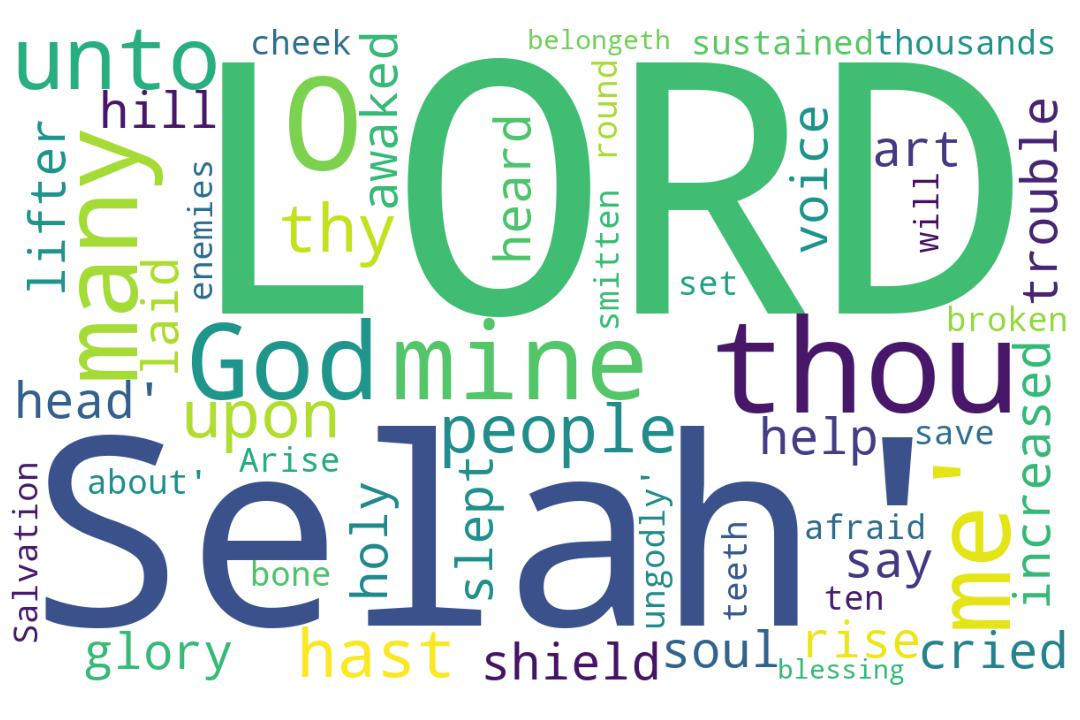
\includegraphics[width=\linewidth]{19OT-Psalms/Psalm3-WordCloud.jpg}
  \caption{Psalm 3 Word Cloud}
  \label{fig:Psalm 3 word Cloud}
\end{figure}

\marginpar{\scriptsize \centering \fcolorbox{bone}{lime}{\textbf{THE LORD, MY HELP}}\\ (Psalm 3:1-8) \begin{compactenum}[I.][8]
	\item A \textbf{Distressed Soul} \index [scripture]{Psalms!Psa 003:02} (Psa 3:2)
	\item A \textbf{Durable Shield} \index [scripture]{Psalms!Psa 003:03} (Psa 3:3)
	\item A \textbf{Defender \& Sustainer} \index[scripture]{Psalms!Psa 003:05} (Psa 3:5)
    \item \textbf{Delightful Sleep} of Peace \index[scripture]{Psalms!Psa 003:05} (Psa 3:5)
    \item One \textbf{Dependable \& Sure} \index[scripture]{Psalms!Psa 003:06} (Psa 3:6)
    \item \textbf{Determined \& Smiting} \index[scripture]{Psalms!Psa 003:07} (Psa 3:7)
   \item  \textbf{Deliverer of Salvation} \index[scripture]{Psalms!Psa 003:08} (Psa 3:8)
\end{compactenum} }

\marginpar{\scriptsize \centering \fcolorbox{bone}{yellow}{\textbf{WHAT GOD DID FOR DAVID}}\\ (Psalm 3:1-8) God:
\begin{compactenum}[I.][8] 
    \item \textbf{God Saw him Surrounded by Enemies} \index[scripture]{Psalms!Psa 003:01} (Psa 3:1)
    \item \textbf{God Secured Him Against Overwhelming Odds} \index[scripture]{Psalms!Psa 003:01} (Psa 3:1)
    \item \textbf{God Sent him Help} \index[scripture]{Psalms!Psa 003:02} (Psa 3:2)
    \item \textbf{God Shielded him from Hurt} \index[scripture]{Psalms!Psa 003:03} (Psa 3:3)
    \item \textbf{God Sustained Him} \index[scripture]{Psalms!Psa 003:05} (Psa 3:5)
    \item \textbf{God Smote the Heathen} \index[scripture]{Psalms!Psa 003:07} (Psa 3:7)
    \item \textbf{God Separated the Teeth of the ungodly} \index[scripture]{Psalms!Psa 003:07} (Psa 3:7)
\end{compactenum} }

\marginpar{\scriptsize \centering \fcolorbox{bone}{black}{\textbf{\textcolor[cmyk]{0,0,0,0}{A TIME OF ANGUISH}}}\\ (Psalm 3) 
\begin{compactenum}[I.]
    \item \textbf{Personal Heartache} - - and heartbreak, but by God's grace and mercy, it was also a time of:
    \item \textbf{Persistent Help} (verses 3, 4, 5, 7)
    \item \textbf{Protected Head} - - God protected both David's physical head and David's throne, the headship as king (verse 3)
    \item A \textbf{Penitential Heart} - - no doubt that David fully realized that Absalom's rebellion, along with many other family problems, results from his sin with Bathsheba. David was never the same after this succession of sin.  He lived with his sorrow.
    \item \textbf{Purifying and Healing} - - there is nothing like God letting us reap the seed we have sown to let us experience his mercy. It is both a purifying and healing process to go through this.  God delivers and cleanses, yet again. 
    \item \textbf{Preserved Honor} - - David gets restored back to the throne, and Absalom is killed by Joab
    \item An \textbf{Ever-Present Hope}
\end{compactenum} }

\marginpar{\scriptsize \centering \fcolorbox{bone}{blue}{\textbf{\textcolor[cmyk]{0,0,0,0}{READYING THE PLACE}}}\\
\fcolorbox{bone}{blue}{\textbf{\textcolor[cmyk]{0,0,0,0}{OF REFUGE}}} \\(Psalm 3) \\
Psalm 3 has the second mention of this word ``Selah''. The first is in 2 Kings 14:7, where it is captured and given the name ``Joktheel.''
\begin{compactenum}[I.]
    \item The \textbf{Capture} - \index[scripture]{2Kings!2Ki 14:07} (2 Kings 14:7)
    \item The \textbf{Coalition} - \index[scripture]{Psalms!Psa 003:01} (Psa 3:1)
    \item The \textbf{Condition} - \index[scripture]{Psalms!Psa 003:02} (Psa 3:2)
    \item The \textbf{Cry} - \index[scripture]{Psalms!Psa 003:04} (Psa 3:4)
    \item The \textbf{Care} - \index[scripture]{Psalms!Psa 003:04} (Psa 3:5)
     \item The \textbf{Conquest} - \index[scripture]{Psalms!Psa 003:07} (Psa 3:7)
   \item The \textbf{Consummation} - \index[scripture]{Psalms!Psa 003:08} (Psa 3:8)
\end{compactenum} }

\footnote{\textcolor[cmyk]{0.99998,1,0,0}{\hyperlink{TOC}{Return to end of Table of Contents.}}}\footnote{\href{https://www.audioverse.org/english/audiobibles/books/ENGKJV/O/Ps/1}{\textcolor[cmyk]{0.99998,1,0,0}{Psalms Audio}}}\textcolor[cmyk]{0.99998,1,0,0}{A Psalm of David, when he fled from Absalom his son.}\\
\\
\textcolor[cmyk]{0.99998,1,0,0}{LORD\textcolor{jungle}{$_{337}$}, how are they increased that trouble me! many \emph{are} they that rise up against me.}
[2] \textcolor[cmyk]{0.99998,1,0,0}{Many\textcolor{jungle}{$_{353}$} \emph{there} \emph{be} which say of my \fcolorbox{bone}{lime}{soul}, \emph{There} \emph{is} no help for him in God. Selah.}
[3] \textcolor[cmyk]{0.99998,1,0,0}{But\textcolor{jungle}{$_{370}$} thou, O LORD, \emph{art} a \fcolorbox{bone}{lime}{shield} for me; my glory, and the lifter up of mine head.}
[4] \textcolor[cmyk]{0.99998,1,0,0}{I\textcolor{jungle}{$_{388}$} cried unto the LORD with my voice, and he heard me out of his holy hill. Selah.}
[5] \textcolor[cmyk]{0.99998,1,0,0}{I\textcolor{jungle}{$_{406}$} laid me down and \fcolorbox{bone}{lime}{slept}; I awaked; for the LORD \fcolorbox{bone}{lime}{sustained} me.}
[6] \textcolor[cmyk]{0.99998,1,0,0}{I\textcolor{jungle}{$_{419}$} will \fcolorbox{bone}{lime}{not} be afraid of ten thousands of people, that have set \emph{themselves} against me round about.}
[7] \textcolor[cmyk]{0.99998,1,0,0}{Arise\textcolor{jungle}{$_{437}$}, O LORD; save me, O my God: for thou hast \fcolorbox{bone}{lime}{smitten} all mine enemies \emph{upon} the cheek bone; thou hast broken the teeth of the ungodly.}
[8] \textcolor[cmyk]{0.99998,1,0,0}{\fcolorbox{bone}{lime}{Salvation}\textcolor{jungle}{$_{464}$} \emph{belongeth} unto the LORD: thy blessing \emph{is} upon thy people. Selah\textcolor{jungle}{$_{475}$}.}



\section{Psalm 3 Comments}




%\index[NWIV]{16!Psalms!Psa 3:1}\index[AWIP]{LORD!Psalms!Psa 3:1}\index[AWIP]{how!Psalms!Psa 3:1}\index[AWIP]{are!Psalms!Psa 3:1}\index[AWIP]{they!Psalms!Psa 3:1}\index[AWIP]{they!Psalms!Psa 3:1 (2)}\index[AWIP]{increased!Psalms!Psa 3:1}\index[AWIP]{that!Psalms!Psa 3:1}\index[AWIP]{that!Psalms!Psa 3:1 (2)}\index[AWIP]{trouble!Psalms!Psa 3:1}\index[AWIP]{me!!Psalms!Psa 3:1}\index[AWIP]{many!Psalms!Psa 3:1}\index[AWIP]{\emph{are}!Psalms!Psa 3:1}\index[AWIP]{rise!Psalms!Psa 3:1}\index[AWIP]{up!Psalms!Psa 3:1}\index[AWIP]{against!Psalms!Psa 3:1}\index[AWIP]{me!Psalms!Psa 3:1}\index[AWIP]{\emph{are}!Psalms!Psa 3:1}

\index[NWIV]{17!Psalms!Psa 3:2}\index[AWIP]{Many!Psalms!Psa 3:2}\index[AWIP]{\emph{there}!Psalms!Psa 3:2}\index[AWIP]{\emph{be}!Psalms!Psa 3:2}\index[AWIP]{which!Psalms!Psa 3:2}\index[AWIP]{say!Psalms!Psa 3:2}\index[AWIP]{of!Psalms!Psa 3:2}\index[AWIP]{my!Psalms!Psa 3:2}\index[AWIP]{soul!Psalms!Psa 3:2}\index[AWIP]{\emph{There}!Psalms!Psa 3:2}\index[AWIP]{\emph{is}!Psalms!Psa 3:2}\index[AWIP]{no!Psalms!Psa 3:2}\index[AWIP]{help!Psalms!Psa 3:2}\index[AWIP]{for!Psalms!Psa 3:2}\index[AWIP]{him!Psalms!Psa 3:2}\index[AWIP]{in!Psalms!Psa 3:2}\index[AWIP]{God!Psalms!Psa 3:2}\index[AWIP]{Selah!Psalms!Psa 3:2}\index[AWIP]{\emph{there}!Psalms!Psa 3:2}\index[AWIP]{\emph{be}!Psalms!Psa 3:2}\index[AWIP]{\emph{There}!Psalms!Psa 3:2}\index[AWIP]{\emph{is}!Psalms!Psa 3:2}

\index[NWIV]{18!Psalms!Psa 3:3}\index[AWIP]{But!Psalms!Psa 3:3}\index[AWIP]{thou!Psalms!Psa 3:3}\index[AWIP]{O!Psalms!Psa 3:3}\index[AWIP]{LORD!Psalms!Psa 3:3}\index[AWIP]{\emph{art}!Psalms!Psa 3:3}\index[AWIP]{a!Psalms!Psa 3:3}\index[AWIP]{shield!Psalms!Psa 3:3}\index[AWIP]{for!Psalms!Psa 3:3}\index[AWIP]{me!Psalms!Psa 3:3}\index[AWIP]{my!Psalms!Psa 3:3}\index[AWIP]{glory!Psalms!Psa 3:3}\index[AWIP]{and!Psalms!Psa 3:3}\index[AWIP]{the!Psalms!Psa 3:3}\index[AWIP]{lifter!Psalms!Psa 3:3}\index[AWIP]{up!Psalms!Psa 3:3}\index[AWIP]{of!Psalms!Psa 3:3}\index[AWIP]{mine!Psalms!Psa 3:3}\index[AWIP]{head!Psalms!Psa 3:3}\index[AWIP]{\emph{art}!Psalms!Psa 3:3}

\index[NWIV]{18!Psalms!Psa 3:4}\index[AWIP]{I!Psalms!Psa 3:4}\index[AWIP]{cried!Psalms!Psa 3:4}\index[AWIP]{unto!Psalms!Psa 3:4}\index[AWIP]{the!Psalms!Psa 3:4}\index[AWIP]{LORD!Psalms!Psa 3:4}\index[AWIP]{with!Psalms!Psa 3:4}\index[AWIP]{my!Psalms!Psa 3:4}\index[AWIP]{voice!Psalms!Psa 3:4}\index[AWIP]{and!Psalms!Psa 3:4}\index[AWIP]{he!Psalms!Psa 3:4}\index[AWIP]{heard!Psalms!Psa 3:4}\index[AWIP]{me!Psalms!Psa 3:4}\index[AWIP]{out!Psalms!Psa 3:4}\index[AWIP]{of!Psalms!Psa 3:4}\index[AWIP]{his!Psalms!Psa 3:4}\index[AWIP]{holy!Psalms!Psa 3:4}\index[AWIP]{hill!Psalms!Psa 3:4}\index[AWIP]{Selah!Psalms!Psa 3:4}

\index[NWIV]{13!Psalms!Psa 3:5}\index[AWIP]{I!Psalms!Psa 3:5}\index[AWIP]{I!Psalms!Psa 3:5 (2)}\index[AWIP]{laid!Psalms!Psa 3:5}\index[AWIP]{me!Psalms!Psa 3:5}\index[AWIP]{me!Psalms!Psa 3:5 (2)}\index[AWIP]{down!Psalms!Psa 3:5}\index[AWIP]{and!Psalms!Psa 3:5}\index[AWIP]{slept!Psalms!Psa 3:5}\index[AWIP]{awaked!Psalms!Psa 3:5}\index[AWIP]{for!Psalms!Psa 3:5}\index[AWIP]{the!Psalms!Psa 3:5}\index[AWIP]{LORD!Psalms!Psa 3:5}\index[AWIP]{sustained!Psalms!Psa 3:5}

\index[NWIV]{18!Psalms!Psa 3:6}\index[AWIP]{I!Psalms!Psa 3:6}\index[AWIP]{will!Psalms!Psa 3:6}\index[AWIP]{not!Psalms!Psa 3:6}\index[AWIP]{be!Psalms!Psa 3:6}\index[AWIP]{afraid!Psalms!Psa 3:6}\index[AWIP]{of!Psalms!Psa 3:6}\index[AWIP]{of!Psalms!Psa 3:6 (2)}\index[AWIP]{ten!Psalms!Psa 3:6}\index[AWIP]{thousands!Psalms!Psa 3:6}\index[AWIP]{people!Psalms!Psa 3:6}\index[AWIP]{that!Psalms!Psa 3:6}\index[AWIP]{have!Psalms!Psa 3:6}\index[AWIP]{set!Psalms!Psa 3:6}\index[AWIP]{\emph{themselves}!Psalms!Psa 3:6}\index[AWIP]{against!Psalms!Psa 3:6}\index[AWIP]{me!Psalms!Psa 3:6}\index[AWIP]{round!Psalms!Psa 3:6}\index[AWIP]{about!Psalms!Psa 3:6}\index[AWIP]{\emph{themselves}!Psalms!Psa 3:6}

\index[NWIV]{27!Psalms!Psa 3:7}\index[AWIP]{Arise!Psalms!Psa 3:7}\index[AWIP]{O!Psalms!Psa 3:7}\index[AWIP]{O!Psalms!Psa 3:7 (2)}\index[AWIP]{LORD!Psalms!Psa 3:7}\index[AWIP]{save!Psalms!Psa 3:7}\index[AWIP]{me!Psalms!Psa 3:7}\index[AWIP]{my!Psalms!Psa 3:7}\index[AWIP]{God!Psalms!Psa 3:7}\index[AWIP]{for!Psalms!Psa 3:7}\index[AWIP]{thou!Psalms!Psa 3:7}\index[AWIP]{thou!Psalms!Psa 3:7 (2)}\index[AWIP]{hast!Psalms!Psa 3:7}\index[AWIP]{hast!Psalms!Psa 3:7 (2)}\index[AWIP]{smitten!Psalms!Psa 3:7}\index[AWIP]{all!Psalms!Psa 3:7}\index[AWIP]{mine!Psalms!Psa 3:7}\index[AWIP]{enemies!Psalms!Psa 3:7}\index[AWIP]{\emph{upon}!Psalms!Psa 3:7}\index[AWIP]{the!Psalms!Psa 3:7}\index[AWIP]{the!Psalms!Psa 3:7 (2)}\index[AWIP]{the!Psalms!Psa 3:7 (3)}\index[AWIP]{cheek!Psalms!Psa 3:7}\index[AWIP]{bone!Psalms!Psa 3:7}\index[AWIP]{broken!Psalms!Psa 3:7}\index[AWIP]{teeth!Psalms!Psa 3:7}\index[AWIP]{of!Psalms!Psa 3:7}\index[AWIP]{ungodly!Psalms!Psa 3:7}\index[AWIP]{\emph{upon}!Psalms!Psa 3:7}

\index[NWIV]{12!Psalms!Psa 3:8}\index[AWIP]{Salvation!Psalms!Psa 3:8}\index[AWIP]{\emph{belongeth}!Psalms!Psa 3:8}\index[AWIP]{unto!Psalms!Psa 3:8}\index[AWIP]{the!Psalms!Psa 3:8}\index[AWIP]{LORD!Psalms!Psa 3:8}\index[AWIP]{thy!Psalms!Psa 3:8}\index[AWIP]{thy!Psalms!Psa 3:8 (2)}\index[AWIP]{blessing!Psalms!Psa 3:8}\index[AWIP]{\emph{is}!Psalms!Psa 3:8}\index[AWIP]{upon!Psalms!Psa 3:8}\index[AWIP]{people!Psalms!Psa 3:8}\index[AWIP]{Selah!Psalms!Psa 3:8}\index[AWIP]{\emph{belongeth}!Psalms!Psa 3:8}\index[AWIP]{\emph{is}!Psalms!Psa 3:8}


\section{Psalm 3 Outlines}

\subsection{My Outlines}

\subsubsection{The Lord, My Help}
\index[speaker]{Keith Anthony!Psalm 003 (The Lord, My Help)}
\index[series]{Psalms (Keith Anthony)!Psalm 003 (The Lord, My Help)}
\index[date]{2014/11/03!Psalm 003 (The Lord, My Help) (Keith Anthony)}

\begin{compactenum}[I.][9]
	\item A \textbf{Distressed Soul} \index [scripture]{Psalms!Psa 003:02} (Psa 3:2)
	\item A \textbf{Durable Shield} \index [scripture]{Psalms!Psa 003:03} (Psa 3:3)
	\item A \textbf{Defender \& Sustainer} \index[scripture]{Psalms!Psa 003:05} (Psa 3:5)
    \item \textbf{The Delightful Sleep} of Peace \index[scripture]{Psalms!Psa 003:05} (Psa 3:5)
    \item One \textbf{Dependable \& Sure} \index[scripture]{Psalms!Psa 003:06} (Psa 3:6)
    \item A \textbf{Determined \& Smiting} \index[scripture]{Psalms!Psa 003:07} (Psa 3:7)
   \item The \textbf{Deliverer of Salvation} \index[scripture]{Psalms!Psa 003:08} (Psa 3:8)
\end{compactenum}

\subsubsection{What God Did for David}

\index[speaker]{Keith Anthony!Psalm 003 (What God Did for David)}
\index[series]{Psalms (Keith Anthony)!Psalm 003 (What God Did for David)}
\index[date]{2014/11/03!Psalm 003 (What God Did for David) (Keith Anthony)}
\textbf{Introduction: }Commentators remind us that Psalm 3 recounts God's protection of David during Absalom's rebellion: 

\begin{compactenum}[I.]
    \item \textbf{God Saw him Surrounded by Enemies} \index[scripture]{Psalms!Psa 003:01} (Psa 3:1)
    \item \textbf{God Secured Him Against Overwhelming Odds} \index[scripture]{Psalms!Psa 003:01} (Psa 3:1)
    \item \textbf{God Sent him Help} \index[scripture]{Psalms!Psa 003:02} (Psa 3:2)
    \item \textbf{God Shielded him from Hurt} \index[scripture]{Psalms!Psa 003:03} (Psa 3:3)
    \item \textbf{God Sustained Him} \index[scripture]{Psalms!Psa 003:05} (Psa 3:5)
    \item \textbf{God Smote the Heathen} \index[scripture]{Psalms!Psa 003:07} (Psa 3:7)
    \item \textbf{God Separated the Teeth of the ungodly} \index[scripture]{Psalms!Psa 003:07} (Psa 3:7)
\end{compactenum}

\subsubsection{A Time of Anguish}
\index[speaker]{Keith Anthony!Psalm 003 (A Time of Anguish)}
\index[series]{Psalms (Keith Anthony)!Psalm 003 (A Time of Anguish)}
\index[date]{2014/11/03!Psalm 003 (A Time of Anguish) (Keith Anthony)}
Commentators remind us that Psalm 3 recounts God's protection of David during Absalom's rebellion. (See the story in 2 Samuel 15:13-17:22). This was a time of: 

\begin{compactenum}[I.]
    \item \textbf{Personal Heartache} - - and heartbreak, but by God's grace and mercy, it was also a time of:
    \item \textbf{Persistent Help} (verses 3, 4, 5, 7)
    \item \textbf{Protected Head} - - God protected both David's physical head and David's throne, the headship as king (verse 3)
    \item A \textbf{Penitential Heart} - - no doubt that David fully realized that Absalom's rebellion, along with many other family problems, results from his sin with Bathsheba. David was never the same after this succession of sin.  He lived with his sorrow.
    \item \textbf{Purifying and Healing} - - there is nothing like God letting us reap the seed we have sown to let us experience his mercy. It is both a purifying and healing process to go through this.  God delivers and cleanses, yet again. 
    \item \textbf{Preserved Honor} - - David gets restored back to the throne, and Absalom is killed by Joab
    \item An \textbf{Ever-Present Hope}
\end{compactenum}


\subsubsection{Readying the Place of Refuge}
\index[speaker]{Keith Anthony!Psalm 003 (Readying the Place of Refuge)}
\index[series]{Psalms (Keith Anthony)!Psalm 003 (Readying the Place of Refuge)}
\index[date]{2021/01/03!Psalm 003 (Readying the Place of Refuge) (Keith Anthony)}

\begin{compactenum}[I.]
    \item The \textbf{Capture} - \index[scripture]{2Kings!2Ki 14:07} (2 Kings 14:7)
    \item The \textbf{Coalition} - \index[scripture]{Psalms!Psa 003:01} (Psa 3:1)
    \item The \textbf{Condition} - \index[scripture]{Psalms!Psa 003:02} (Psa 3:2)
    \item The \textbf{Cry} - \index[scripture]{Psalms!Psa 003:04} (Psa 3:4)
    \item The \textbf{Care} - \index[scripture]{Psalms!Psa 003:04} (Psa 3:5)
     \item The \textbf{Conquest} - \index[scripture]{Psalms!Psa 003:07} (Psa 3:7)
   \item The \textbf{Consummation} - \index[scripture]{Psalms!Psa 003:08} (Psa 3:8)
\end{compactenum} 

\subsection{Outlines from Others}

\subsubsection{David at Mananaim}\footnote{John Phillips}
From John Phillips\cite{Phillips2001ExploringPsalms1}
\begin{compactenum}[I.]
    \item \textbf{David's Trial} (Psalm 3:1-2)
    \begin{compactenum}[A.]
        \item The Multiplicity of His Foes (Psalm 3:1)
        \item The Malignity of His Foes (Psalm 3:1)
    \end{compactenum}
    \item \textbf{David's Trust} (Psalm 3:3-4)
    \begin{compactenum}[A.]
        \item His Assurance in God (Psalm 3:3)
        \item His Appeal to God (Psalm 3:4)
    \end{compactenum}
    \item \textbf{David's Triumph} (Psalm 3:5-8)
    \begin{compactenum}[A.]
        \item David's Vision (Psalm 3:5-6)
        \item David's Victory (Psalm 3:7-8)
    \end{compactenum}
\end{compactenum}
\newpage



%\section{Psalm 3 Statistics}

%%%%%%%%%%%%%%%%%%%%%%%%%%%
%%%%%Word Statistics
%%%%%%%%%%%%%%%%%%%%%%%%%%%


\normalsize



\subsection{Chapter Word Statistics}


%%%%%%%%%%
%%%%%%%%%%
 
\begin{center}
\begin{longtable}{l|c|c|c|c}
\caption[Stats for Psalm 3]{Stats for Psalm 3} \label{table:Stats for Psalm 3} \\ 
\hline \multicolumn{1}{|c|}{\textbf{Verse(s)}} & \multicolumn{1}{|c|}{\textbf{Count}} & \multicolumn{1}{|c|}{\textbf{Unique}} & \multicolumn{1}{|c|}{\textbf{Italics}} & \multicolumn{1}{|c|}{\textbf{Uniq Italic}}  \\ \hline 
\endfirsthead
 
\multicolumn{5}{c}
{{\bfseries \tablename\ \thetable{} -- continued from previous page}} \\  
\hline \multicolumn{1}{|c|}{\textbf{Verse(s)}} & \multicolumn{1}{|c|}{\textbf{Count}} & \multicolumn{1}{|c|}{\textbf{Unique}} & \multicolumn{1}{|c|}{\textbf{Italics}} & \multicolumn{1}{|c|}{\textbf{Uniq Italic}}  \\ \hline 
\endhead
 
\hline \multicolumn{5}{|r|}{{Continued if needed}} \\ \hline
\endfoot 
1 & 16 & 13 & 1 & 1\\ \hline
2 & 17 & 17 & 4 & 4\\ \hline
3 & 18 & 18 & 1 & 1\\ \hline
4 & 18 & 18 & 0 & 0\\ \hline
5 & 13 & 11 & 0 & 0\\ \hline
6 & 18 & 17 & 1 & 1\\ \hline
7 & 27 & 22 & 1 & 1\\ \hline
8 & 12 & 11 & 2 & 2\\ \hline
\hline \hline
Total & 139 & 87 & 10 & 9



\end{longtable}
\end{center}

%%%%%%%%%%
%%%%%%%%%%
 
\subsection{Words by Frequency}

\begin{center}
\begin{longtable}{l|r}
\caption[Word Frequencies in Psalm 3]{Word Frequencies in Psalm 3} \label{table:WordsIn-Psalm-3} \\ 
\hline \multicolumn{1}{|c|}{\textbf{Word}} & \multicolumn{1}{c|}{\textbf{Frequency}} \\ \hline 
\endfirsthead
 
\multicolumn{2}{c}
{{\bfseries \tablename\ \thetable{} -- continued from previous page}} \\ 
\hline \multicolumn{1}{|c|}{\textbf{Word}} & \multicolumn{1}{c|}{\textbf{Frequency}} \\ \hline 
\endhead
 
\hline \multicolumn{2}{|r|}{{Continued if needed}} \\ \hline
\endfoot
 
\hline \hline
\endlastfoot
me & 8 \\ \hline
the & 7 \\ \hline
LORD & 6 \\ \hline
of & 6 \\ \hline
my & 4 \\ \hline
for & 4 \\ \hline
I & 4 \\ \hline
that & 3 \\ \hline
Selah & 3 \\ \hline
thou & 3 \\ \hline
O & 3 \\ \hline
and & 3 \\ \hline
they & 2 \\ \hline
up & 2 \\ \hline
against & 2 \\ \hline
\emph{is} & 2 \\ \hline
God & 2 \\ \hline
mine & 2 \\ \hline
unto & 2 \\ \hline
people & 2 \\ \hline
hast & 2 \\ \hline
thy & 2 \\ \hline
how & 1 \\ \hline
are & 1 \\ \hline
increased & 1 \\ \hline
trouble & 1 \\ \hline
many & 1 \\ \hline
\emph{are} & 1 \\ \hline
rise & 1 \\ \hline
Many & 1 \\ \hline
\emph{there} & 1 \\ \hline
\emph{be} & 1 \\ \hline
which & 1 \\ \hline
say & 1 \\ \hline
soul & 1 \\ \hline
\emph{There} & 1 \\ \hline
no & 1 \\ \hline
help & 1 \\ \hline
him & 1 \\ \hline
in & 1 \\ \hline
But & 1 \\ \hline
\emph{art} & 1 \\ \hline
a & 1 \\ \hline
shield & 1 \\ \hline
glory & 1 \\ \hline
lifter & 1 \\ \hline
head & 1 \\ \hline
cried & 1 \\ \hline
with & 1 \\ \hline
voice & 1 \\ \hline
he & 1 \\ \hline
heard & 1 \\ \hline
out & 1 \\ \hline
his & 1 \\ \hline
holy & 1 \\ \hline
hill & 1 \\ \hline
laid & 1 \\ \hline
down & 1 \\ \hline
slept & 1 \\ \hline
awaked & 1 \\ \hline
sustained & 1 \\ \hline
will & 1 \\ \hline
not & 1 \\ \hline
be & 1 \\ \hline
afraid & 1 \\ \hline
ten & 1 \\ \hline
thousands & 1 \\ \hline
have & 1 \\ \hline
set & 1 \\ \hline
\emph{themselves} & 1 \\ \hline
round & 1 \\ \hline
about & 1 \\ \hline
Arise & 1 \\ \hline
save & 1 \\ \hline
smitten & 1 \\ \hline
all & 1 \\ \hline
enemies & 1 \\ \hline
\emph{upon} & 1 \\ \hline
cheek & 1 \\ \hline
bone & 1 \\ \hline
broken & 1 \\ \hline
teeth & 1 \\ \hline
ungodly & 1 \\ \hline
Salvation & 1 \\ \hline
\emph{belongeth} & 1 \\ \hline
blessing & 1 \\ \hline
upon & 1 \\ \hline
\end{longtable}
\end{center}



\normalsize



\subsection{Words Alphabetically}

\begin{center}
\begin{longtable}{l|r}
\caption[Word Alphabetically in Psalm 3]{Word Alphabetically in Psalm 3} \label{table:WordsIn-Psalm-3} \\ 
\hline \multicolumn{1}{|c|}{\textbf{Word}} & \multicolumn{1}{c|}{\textbf{Frequency}} \\ \hline 
\endfirsthead
 
\multicolumn{2}{c}
{{\bfseries \tablename\ \thetable{} -- continued from previous page}} \\ 
\hline \multicolumn{1}{|c|}{\textbf{Word}} & \multicolumn{1}{c|}{\textbf{Frequency}} \\ \hline 
\endhead
 
\hline \multicolumn{2}{|r|}{{Continued if needed}} \\ \hline
\endfoot
 
\hline \hline
\endlastfoot
Arise & 1 \\ \hline
But & 1 \\ \hline
God & 2 \\ \hline
I & 4 \\ \hline
LORD & 6 \\ \hline
Many & 1 \\ \hline
O & 3 \\ \hline
Salvation & 1 \\ \hline
Selah & 3 \\ \hline
\emph{There} & 1 \\ \hline
\emph{are} & 1 \\ \hline
\emph{art} & 1 \\ \hline
\emph{belongeth} & 1 \\ \hline
\emph{be} & 1 \\ \hline
\emph{is} & 2 \\ \hline
\emph{themselves} & 1 \\ \hline
\emph{there} & 1 \\ \hline
\emph{upon} & 1 \\ \hline
a & 1 \\ \hline
about & 1 \\ \hline
afraid & 1 \\ \hline
against & 2 \\ \hline
all & 1 \\ \hline
and & 3 \\ \hline
are & 1 \\ \hline
awaked & 1 \\ \hline
be & 1 \\ \hline
blessing & 1 \\ \hline
bone & 1 \\ \hline
broken & 1 \\ \hline
cheek & 1 \\ \hline
cried & 1 \\ \hline
down & 1 \\ \hline
enemies & 1 \\ \hline
for & 4 \\ \hline
glory & 1 \\ \hline
hast & 2 \\ \hline
have & 1 \\ \hline
he & 1 \\ \hline
head & 1 \\ \hline
heard & 1 \\ \hline
help & 1 \\ \hline
hill & 1 \\ \hline
him & 1 \\ \hline
his & 1 \\ \hline
holy & 1 \\ \hline
how & 1 \\ \hline
in & 1 \\ \hline
increased & 1 \\ \hline
laid & 1 \\ \hline
lifter & 1 \\ \hline
many & 1 \\ \hline
me & 8 \\ \hline
mine & 2 \\ \hline
my & 4 \\ \hline
no & 1 \\ \hline
not & 1 \\ \hline
of & 6 \\ \hline
out & 1 \\ \hline
people & 2 \\ \hline
rise & 1 \\ \hline
round & 1 \\ \hline
save & 1 \\ \hline
say & 1 \\ \hline
set & 1 \\ \hline
shield & 1 \\ \hline
slept & 1 \\ \hline
smitten & 1 \\ \hline
soul & 1 \\ \hline
sustained & 1 \\ \hline
teeth & 1 \\ \hline
ten & 1 \\ \hline
that & 3 \\ \hline
the & 7 \\ \hline
they & 2 \\ \hline
thou & 3 \\ \hline
thousands & 1 \\ \hline
thy & 2 \\ \hline
trouble & 1 \\ \hline
ungodly & 1 \\ \hline
unto & 2 \\ \hline
up & 2 \\ \hline
upon & 1 \\ \hline
voice & 1 \\ \hline
which & 1 \\ \hline
will & 1 \\ \hline
with & 1 \\ \hline
\end{longtable}
\end{center}



\normalsize



\subsection{Word Lengths in Chapter}
\normalsize
\begin{longtable}{l|p{3.75in}}
\caption[Words by Length in Psalm 3]{Words by Length in Psalm 3} \label{table:WordsIn-Psalm-3} \\ 
\hline \multicolumn{1}{|c|}{\textbf{Length}} & \multicolumn{1}{c|}{\textbf{Words}} \\ \hline 
\endfirsthead
 
\multicolumn{2}{c}
{{\bfseries \tablename\ \thetable{} -- continued from previous page}} \\ 
\hline \multicolumn{1}{|c|}{\textbf{Length}} & \multicolumn{1}{c|}{\textbf{Words}} \\ \hline 
\endhead
 
\hline \multicolumn{2}{|r|}{{Continued if needed}} \\ \hline
\endfoot
 
\hline \hline
\endlastfoot
1 & O, a, I \\ \hline
2 & me, up, \emph{be}, of, my, \emph{is}, no, in, he, be \\ \hline
3 & how, are, \emph{are}, say, for, him, God, But, \emph{art}, and, the, out, his, not, ten, set, all, thy \\ \hline
4 & LORD, they, that, many, rise, Many, soul, help, thou, mine, head, unto, with, holy, hill, laid, down, will, have, save, hast, \emph{upon}, bone, upon \\ \hline
5 & \emph{there}, which, \emph{There}, Selah, glory, cried, voice, heard, slept, round, about, Arise, cheek, teeth \\ \hline
6 & shield, lifter, awaked, afraid, people, broken \\ \hline
7 & trouble, against, smitten, enemies, ungodly \\ \hline
8 & blessing \\ \hline
9 & increased, sustained, thousands, Salvation, \emph{belongeth} \\ \hline
10 & \emph{themselves} \\ \hline
\end{longtable}






%%%%%%%%%%
%%%%%%%%%%
 



%%%%%%%%%%
%%%%%%%%%%
\subsection{Verses with 13 Words in Chapter}
\normalsize
\begin{longtable}{l|p{3.75in}}
\caption[Verses with 13 Words  in Psalm 3]{Verses with 13 Words  in Psalm 3} \label{table:Verses with 13 Words in-Psalm-3} \\ 
\hline \multicolumn{1}{|c|}{\textbf{Reference}} & \multicolumn{1}{c|}{\textbf{Verse}} \\ \hline 
\endfirsthead
 
\multicolumn{2}{c}
{{\bfseries \tablename\ \thetable{} -- continued from previous page}} \\ 
\hline \multicolumn{1}{|c|}{\textbf{Reference}} & \multicolumn{1}{c|}{\textbf{Verse}} \\ \hline 
\endhead
 
\hline \multicolumn{2}{|r|}{{Continued if needed}} \\ \hline
\endfoot
 
\hline \hline
\endlastfoot
Psalms 003:5 & I laid me down and slept; I awaked; for the LORD sustained me. \\ \hline
\end{longtable}






%%%%%%%%%%
%%%%%%%%%%
\subsection{Psalm3 Repeated Phrases}


%%%%%%%%%%
%%%%%%%%%%
\normalsize
 
\begin{center}
\begin{longtable}{|p{3.0in}|p{0.5in}|}
\caption[Psalm3 Repeated Phrases]{Psalm3 Repeated Phrases}\label{table:Repeated Phrases Psalm3} \\
\hline \multicolumn{1}{|c|}{\textbf{Phrase}} & \multicolumn{1}{c|}{\textbf{Frequency}} \\ \hline 
\endfirsthead
 
\multicolumn{2}{c}
{{\bfseries \tablename\ \thetable{} -- continued from previous page}} \\  
\hline \multicolumn{1}{|c|}{\textbf{Phrase}} & \multicolumn{1}{c|}{\textbf{Frequency}} \\ \hline 
\endhead
 
\hline \multicolumn{2}{c}{{ }} \\ \hline
\endfoot 
the LORD & 3\\ \hline 
\end{longtable}
\end{center}



%%%%%%%%%%
%%%%%%%%%%






%\input{Template}
\scriptsize

\chapter{Indices}

\printindex[DOCTRINES]
\printindex[scripture]

\printindex[speaker]
%\printindex[series]

\printindex[FACEBOOK]
\printindex[LOCATION]

\printindex[AWIP]


\printbibliography
\end{document}

